%%
\documentclass[%
]{report}

\usepackage[14pt]{extsizes} % для того чтобы задать нестандартный 14-ый размер шрифта
\usepackage[left=30mm, top=20mm, right=20mm, bottom=30mm, footskip=15mm]{geometry}

\usepackage[utf8]{inputenc}

\usepackage{polyglossia}
\setdefaultlanguage[spelling=modern]{russian}
\setotherlanguages{english}


\usepackage[style=gost-numeric,sorting=none]{biblatex}

\usepackage{graphicx}
\usepackage{tabularx}
\usepackage{longtable}
% \usepackage{booktabs}
\usepackage{ragged2e}

\usepackage[normalem]{ulem}

\usepackage{indentfirst}
\setlength\parindent{1.25cm}

\hyphenpenalty=4000
\exhyphenpenalty=7500

\usepackage{setspace}

\usepackage{caption}
\captionsetup{font=small}

% \usepackage[nolists,figuresonly,fighead]{endfloat}

\usepackage{titlesec}
\usepackage{lipsum}
\usepackage{subcaption}

\titleformat{\chapter}[hang]{\normalfont\LARGE\bfseries}{\thechapter}{1em}{}


\captionsetup[listing]{name=Листинг}

\setmainfont[Ligatures=TeX,Scale=MatchLowercase]{CMU Serif}
\setsansfont[Ligatures=TeX,Scale=MatchLowercase]{CMU Sans Serif}
\setmonofont[Scale=MatchLowercase]{CMU Typewriter Text}

% \usepackage{mathptmx}


% CMU Serif
\newfontfamily\cyrillicfont%
[Script=Cyrillic,Ligatures=TeX,Scale=MatchLowercase]%
{CMU Serif}

% CMU Sans Serif
\newfontfamily\cyrillicfontsf%
[Script=Cyrillic,Ligatures=TeX,Scale=MatchLowercase]%
{CMU Sans Serif}

% CMU Typewriter Text
\newfontfamily\cyrillicfonttt%
[Script=Cyrillic,Scale=MatchLowercase]%
{CMU Typewriter Text}


%%% One can fix some overfulls
\sloppy

%% Minted listings support
%% Need pygment <http://pygments.org/> <http://pypi.python.org/pypi/Pygments>
%\usepackage[newfloat]{minted}
\usepackage{minted}
%% auto break lines
\setminted{breaklines=true}

%\usepackage{caption}

%\newenvironment{code}{\captionsetup{type=listing}}{}
%\SetupFloatingEnvironment{listing}{name=Листинг}

\addbibresource{main.bib}

%% end of the preamble, start of the body of the document source.
\begin{document}

\selectlanguage{russian}

%%
%% Rights management information.
%% CC-BY is default license.
% \copyrightyear{2025}
% \copyrightclause{Copyright for this paper by its authors.
%   Use permitted under Creative Commons License Attribution 4.0
%   International (CC BY 4.0).}

%%
%% This command is for the conference information
% \conference{Information and Telecommunication Technologies and Mathematical Modeling of High-Tech Systems 2025 (ITTMM 2025), Moscow, April 07--11, 2025}

%%
%% The "title" command
\title{Симулятор беспроводной меш-сети для мобильных роботов}
% \title[mode=trans]{Wireless mesh network simulator for mobile robots}



% НАЧАЛО ТИТУЛЬНОГО ЛИСТА
\newgeometry{left=30mm, top=1mm, right=20mm, bottom=1mm}
\begin{titlepage}

  \begin{center}
    \hfill \break
    \small
    \textbf{
      МИНИСТЕРСТВО НАУКИ И ВЫСШЕГО ОБРАЗОВАНИЯ\\
      РОССИЙСКОЙ ФЕДЕРАЦИИ\\
      ФЕДЕРАЛЬНОЕ ГОСУДАРСТВЕННОЕ АВТОНОМНОЕ ОБРАЗОВАТЕЛЬНОЕ\\
      УЧРЕЖДЕНИЕ ВЫСШЕГО ОБРАЗОВАНИЯ\\
      <<РОССИЙСКИЙ УНИВЕРСИТЕТ ДРУЖБЫ НАРОДОВ\\
      ИМЕНИ ПАТРИСА ЛУМУМБЫ>>
    }\\
    \normalsize
    Факультет \uline{физико-математических и естественных наук}\\ 
    Кафедра \uline{математического моделирования и искусственного интеллекта}

    \vspace*{\fill}
 
    \begin{flushright}
      <<Допустить к защите>>\\
      Заведующий кафедрой\\
      математического моделирования\\и искусственного интеллекта\\
      д.ф-м.н., доцент\\
      \underline{\phantom{signature signa}} Малых М.Д.\\
      <<\underline{\phantom{day}}>> \underline{\phantom{month month}} 2025 г.
    \end{flushright}
   
    \vspace*{\fill}
    \Large{\textbf{Выпускная квалификационная работа\\ бакалавра}}
    \\
    \normalsize
    \vspace{0.5cm}
    Направление  09.03.03 <<\uline{Прикладная информатика}>>
  \end{center}

  \vspace*{\fill}

  \begin{justify}
    \mbox{ТЕМА \uline{<<Меш-сеть роя автономных роботов: построение и маршрутизация>>}} \\
    Выполнил студент \underline{\textbf{Генералов Даниил Михайлович}}
  \end{justify}
  
  \vspace*{\fill}

  \noindent\begin{tabular}{p{0.5\linewidth} c}
Группа \uline{НПИбд-01-21} & Руководитель выпускной  \\
      & квалификационной работы\\
      Студ. билет \textnumero{} \underline{1032212280} & \uline{Виноградов Андрей Николаевич,}\\
      & \uline{к.ф.-м.н., доцент кафедры ММиИИ} \\
      \\
      & \underline{\phantom{signature signature signature sig}} \\
      \\
      \\
      & Автор \underline{\phantom{signature signature signat}} \\
    \end{tabular}
   \vspace*{\fill}
   
  \begin{center} \textbf{г. Москва} \\ 2025 г. \end{center}
  \thispagestyle{empty} % выключаем отображение номера для этой страницы
   
  \end{titlepage}
   % КОНЕЦ ТИТУЛЬНОГО ЛИСТА
  %  \renewcommand{\baselinestretch}{1.5}
  \restoregeometry
   \newpage
   \setstretch{1.2}


% \begin{titlepage}
\begin{center}
  \textbf{Федеральное государственное автономное образовательное учреждение высшего образования} \\
  \textbf{<<Российский университет дружбы народов}\\
  \textbf{имени Патриса Лумумбы>>}\\

  \vspace*{\fill}

  \large \textbf{АННОТАЦИЯ}\\
  \normalsize \textbf{выпускной квалификационной работы} \\

  \uline{Генералова Даниила Михайловича}
\end{center}

\noindent на тему: \uline{Меш-сеть роя автономных роботов: построение и маршрутизация}

Данная работа посвящена моделированию и разработке алгоритмов и протоколов
для построения меш-сетей, в особенности для поддержания надежных
постоянных соединений для
использования в роевых сетях мобильных роботов.

В ходе работы разработан симулятор для тестирования поведения мобильных роботов,
оснащенных радио-модулями.
Симулятор запускает скрипты, которые управляют движением каждого робота и
радио-коммуникацией с другими роботами в окружении.
Эти скрипты используют интерфейс,
который легко реализовать на аппаратной платформе,
из-за чего код, разработанный для этого симулятора,
можно без изменений использовать для полевых исследований.

Этот обзор литературы помог определить некоторые частые тенденции в тестировании
и разработке алгоритмов маршрутизации в меш-сетях:
например, что почти все исследования основывают свои выводы на симуляциях.
Данная работа может стать основой для новых исследований,
которые сравнивают различные алгоритмы в контроллируемых условиях,
а также на аппаратных платформах.

\vspace*{\fill}

\noindent \begin{tabular}{p{0.33\linewidth} p{0.33\linewidth} p{0.33\linewidth}}
Автор ВКР & \underline{\phantom{signature sign}} & \underline{\phantom{Генералов Даниил}} \\
& (Подпись) & (ФИО)
\end{tabular}

\thispagestyle{empty} 

% \end{titlepage}
\newpage

\setstretch{1.5}

\setcounter{page}{3}  

\tableofcontents

\newpage

% \tnotemark[1]
% \tnotetext[1]{You can use this document as the template for preparing your publication. We recommend using the latest version of the ittmm style.}

%%
%% The "author" command and its associated commands are used to define
%% the authors and their affiliations.
% \author{Даниил М. Генералов}
% [%
% trans={Daniil M. Generalov},
% orcid=0000-0002-2337-1176,
% email=1032212280@pfur.ru,
% %url=https://yamadharma.github.io/,
% ]
% \cormark[1]

% \address[1]{Российский университет дружбы народов, ул. Миклухо-Маклая, д. 6, Москва, 117198, Российская Федерация}

% \author[1]{Андрей Н. Виноградов}[%
% trans={Andrei N. Vinogradov},
% email=vinogradov-an@rudn.ru,
% orcid=0000-0002-3349-8859,
% ]

%%% Footnotes
% \cortext[1]{Автор, отвечающий за публикацию.}

%%
%% The abstract is a short summary of the work to be presented in the
%% article.
% \begin{abstract}
% В этой работе мы представляем программу-симулятор
% для разработки и тестирования алгоритмов маршрутизации
% в беспроводных меш-сетях на мобильных роботах.
% С помощью этого симулятора можно
% изучать поведение этих мобильных роботов
% при различных условиях радио-связи,
% которые трудно симулировать на физическом оборудовании.
% Код, написанный для симулятора,
% можно использовать на физических микроконтроллерах без изменений.
% Интеграция симуляции радио-связи
% и движения роботов по прямоугольной сетке
% является новым подходом,
% который сложно воспроизвести в существующих инструментах симуляции сетей.
% \end{abstract}

%%
%% Keywords. The author(s) should pick words that accurately describe
%% the work being presented. Separate the keywords with commas.
% \begin{keywords}
%   меш-сеть \sep
%   MANET \sep
%   маршрутизация \sep
%   симулятор
% \end{keywords}

%% This command processes the author and affiliation and title
%% information and builds the first part of the formatted document.
% \maketitle

% \chapter{Введение}
\chapter*{Введение}
\addcontentsline{toc}{chapter}{Введение}
\label{sec:intro}

Данная работа посвещена изучению вопросов маршрутизации в беспроводных меш-сетях,
которые используются для различных ситуаций, где требуется передача информации без использования фиксированной инфраструктуры.
Одна из важных задач применения меш-сетей -- в мобильной робототехнике,
и поэтому работа рассматривает особенности использования меш-сетей в контексте задачи мультиагентного планирования.
В рамках написания статьи был проведен обзор литературы, чтобы понять текущие тенденции в разработке и тестировании
алгоритмов маршрутизации,
а также разработан симулятор,
который позволяет прототипировать алгоритм маршрутизации и планирования.

\section*{Актуальность работы}

По мере роста рынка устройств IoT (<<интернета вещей>>)
в форме сенсорных сетей, промышленных манипуляторов или роев мобильных роботов,
появляется необходимость иметь надежные, отказоустойчивые методы
коммуникации между ними.
Самые простые устройства, которые доступны в потребительском сегменте,
используют Wi-Fi или Bluetooth -- два самых частых радио-протокола,
поддержка которых есть во всех современных смартфонах.

Однако IoT-устройства, работающие по Wi-Fi, зависят от доступности центральной точки доступа (\emph{Access Point}, AP).
Более того, наличие Wi-Fi часто подразумевает наличие интернет-соединения,
и многие IoT-устройства перестают работать, когда интернет недоступен.
Наконец, потребительские Wi-Fi роутеры часто имеют предел устройств, которые могут быть подключены к ним,
и наличие большого количества IoT-клиентов может перегрузить способности сети.

Ввиду этих ограничений, новые IoT-устройства часто производятся с поддержкой других
радио-протоколов, таких как ZigBee~\cite{zigbee-792946} и Matter Thread~\cite{csa2023thread},
которые основаны на другом физическом слое: IEEE 802.15.4~\cite{ieee-lorawan-9144691}.
Они предназначены для полностью локального использования,
и они также имеют поддержку меш-архитектур.
Это позволяет разворачивать такие сети без значительных инфраструктурных вложений.

Для того, чтобы такие системы работали эффективно,
особенно при высокой мобильности или ограниченных бюджетах энергии,
нужно разрабатывать эффективные протоколы маршрутизации в этих сетях,
которые оптимизированны под конкретные требования меш-сети.

\section*{Цель работы}

Целью данной работы является изучение алгоритмов маршрутизации в меш-сетях,
а также разработка симуляционной платформы для разработки и тестирования этих алгоритмов.

\section*{Задачи работы}

\noindent Основными задачами данной работы является:

\begin{enumerate}
  \item Разработка симулятора движения и радио-взаимодействия для мобильных роботов;
  \item Для этого симулятора, создание универсального интерфейса,
  который также можно использовать на аппаратной платформе;
  \item Демонстрация и тестирование алгоритмов маршрутизации на основании разработанного интерфейса.
\end{enumerate}

\section*{Методы исследования}

Для разработки симулятора и алгоритмов, которые запускаются внутри него,
используется язык Rust~\cite{klabnik2022rust,10.1145/2692956.2663188}.
Это позволяет запускать алгоритмы в симуляторе на основе игрового движка Bevy~\cite{bevyengine},
а также на встраиваемых платформах с помощью Embassy~\cite{embassy}.

\section*{Апробация работы}

В ходе выполнения работы были получены результаты, представленные на
всероссийской конференции с международным участием
<<Информационно-телекоммуникационные технологии и математическое моделирование высокотехнологичных систем>> (Москва, РУДН, 2025 г.).


\section*{Публикации}

По теме выпускной квалификационной работы бакалавра была опубликована работа~\cite{ittmm}.

\section*{Структура работы}

Работа состоит из введения, трех глав, заключения и списка литературы.
Во введении отражена проблематика выбранной темы, актуальность этой темы в современном мире, поставлены цели и задачи данной работы.
Первая часть содержит обзор литературных источников, посвященных теме работы.
Вторая часть описывает процесс разработки и тестирования симулятора,
в том числе объясняя связь принятых решений по дизайну с характеристиками и ограничениями физической реализации.
В третьей части симулятор используется для того, чтобы продемонстрировать возможность
реализации на основании приведенных интерфейсов алгоритмов маршрутизации.
В заключении описаны результаты и сделаны выводы по проделанной работе,
предложены способы использования результатов и возможные направления дальнейшей деятельности.

\section*{Справочная информация}


\subsection*{Меш-сети}
Беспроводные меш-сети (MANET, \emph{Mobile Ad-hoc Network})
отличаются от традиционных радио-сетей тем,
что они не имеют центрального роутера (такого как Wi-Fi AP или сотовая базовая станция: такой дизайн также известен как \emph{hub-and-spoke});
вместо этого каждый клиент сети является также роутером для своих соседей.

На таком принципе работают рации:
каждая рация может передать сигнал тем приемникам, которые находятся в ее радиусе действия.
Сообщения могут идти дальше, чем радиус действия одного сигнала,
посредством ретрансляции:
если Алиса хочет передать сообщение Чарли,
но Алиса находится слишком далеко от него,
то Алиса может передать свое сообщение Бобу,
и Боб сможет передать сообщение дальше --
либо напрямую к Чарли, если он находится в его радиусе,
либо кому-то еще, кто находится ближе к Чарли.

Такой способ подключения напоминает широкое устройство интернета:
там тоже нет центральных роутеров,
и вместо этого каждая автономная система (AS, \emph{Autonomous System})
имеет пир-соединения (\emph{peering}) с другими AS.
Для этого администраторы двух сетей
соединяют свои роутеры друг с другом
и настраивают свою сеть так, чтобы обе стороны
могли доставлять свои пакеты через другую AS.

Таким образом сети различных организаций составляют глобальную сеть.
Автономные системы обмениваются информацией о том, какие другие системы доступны им,
с помощью протокола BGP (Border Gateway Protocol),
и на основании этой информации их роутеры решают, куда отправлять приходящий им трафик.

Устройство в беспроводной меш-сети примерно аналогично автономной системе интернета.
Однако есть одно важное отличие:
настройка пир-соединений между AS выполняется вручную
по обоюдному согласию администраторов каждой AS,
требует создания физического подключения
и настройки роутеров внутри AS.
Напротив, в беспроводной меш-сети,
устройства могут двигаться относительно друг друга и менять свою сетевую конфигурацию динамически,
так что настройка соединений между устройствами и обмен информацией
должен происходить без участия человека.

Дополнительная сложность заключается в том, что
беспроводные меш-сети часто используются в ситуациях,
когда каждое устройство имеет ограниченные вычислительные ресурсы.
Автономные системы, особенно крупные,
состоят из мощных роутеров,
которые имеют возможность хранить в памяти всю карту глобального интернета
и быстро использовать ее для поиска маршрутов.
Беспроводные меш-сети, напротив, используются в тех ситуациях,
когда есть задача использовать более простое оборудование,
например смартфоны или даже микроконтроллеры:
они не всегда имеют возможность хранить полную карту своей сети,
и поэтому должны использовать подходы для работы с ограниченными ресурсами.

Меш-сети сложнее для разработки, потому что они требуют
изучения проблем координации вроде задачи византийских генералов на маштабах всей сети --
в то время как если есть централизованная инфраструктура управления, это становится проще.
Но меш-сети очень полезны в ситуациях, когда фиксированные сети недоступны или ненадежны:
например, при поисково-спасательных работах или при нарушении инфраструктуры электропитания.

Уже существуют проекты для симуляции маршрутизации в фиксированных сетях:
например, GNS3, OMNeT++~\cite{9181563} и Cisco PacketTracer.
Но с помощью таких проектов сложно сделать симуляцию беспроводной меш-сети,
особенно основанной на подвижных роботах:
эти программы ожидают, что пользователь настроит все проводные соединения
во время моделирования,
и динамическое изменение соединений в них более сложно или невозможно,
и в любом случае требует ручного ввода.

Также существуют некоторые алгоритмы для маршрутизации,
которые специализированны для меш-сетей
(например, OLSR и B.A.T.M.A.N~\cite{DBLP:journals/corr/abs-1901-02298}).
С помощью симулятора можно проверять устойчивость этих алгоритмов к меняющимся условиям,
определить возможные патологические случаи
и изучать возможные улучшения
в контроллируемой среде.
Симулятор, разработанный для этой работы,
имеет отличительную характеристику,
что код, написанный для него,
может быть использован на аппаратной платформе без изменений:
такие существуют только для определенных программных платформ, например Cooja для Contiki-NG~\cite{Contiki-NG}.

\subsection*{Мультиагентное планирование}

Мультиагентное планирование (MAP, \emph{Multi-Agent Planning}) --
это расширение классической задачи планирования
на множество агентов.

Обычная задача планирования состоит из двух частей:
\emph{domain} (область действия) и \emph{problem} (задача).
В domain описываются типы предметов, которые существуют,
предикаты, которые могут быть использованы в задаче,
и возможные действия (каждое из которых задается как комбинация предусловия и постусловия).

В problem описывается набор конкретных предметов,
начальное состояние мира (как множество предикатов),
а также целевое состояние -- набор предикатов, таких, что
после выполнения плана мир будет иметь данные предикаты.

Есть несколько разных определений задачи мультиагентного планирования.
Самое частое определение (согласно~\cite{doi:10.3233/MGS-2009-0133}),
которое принято в данной работе, --
что в мультиагентном планировании
все агенты имеют общий domain,
а также общую информацию о начальном состоянии,
но они могут иметь разные цели.
Агенты не могут говорить друг другу о своих целях:
вместо этого они предлагают планы,
и другие агенты соглашаются или отказываются от него.

Дополнительное усложнение задачи --
когда информация о начальном состоянии не полная,
и наблюдения могут противоречить этим данным.
В таком случае агенты должны остановиться в выполнении плана
и обсудить, что делать дальше:
возможно, новая информация приведет к тому, что план нужно будет перестроить.

В контексте данной работы, меш-сеть делается для обеспечения коммуникации между роботами,
которые решают задачу мультиагентного планирования.
Хотя в общем случае модуль работы с меш-сетью можно использовать отдельно,
в данной работе также интересно рассмотреть взаимодействие этих частей:
например, робот может отказаться выполнять план,
который приведет к тому, что он окажется изолированным от других роботов.


\chapter{Обзор литературы о существующих методах}

В этом обзоре литературы мы
систематически анализируем существующие методологии
и пробелы в областях исследований,
следуя шаблону PRISMA-ScR~\cite{prisma-src}.
Обзор обращает особое внимание на
существующие протоколы маршрутизации,
метрики оценки их эффективности и практически применения их.
Цель -- предоставить основу для будущих разработках
масштабируемых, эффективных и адаптируемых
MANET-сетей,
позволяя их использование в широком спектре IoT-задач.

Основные цели этого обзорного исследования заключаются в:

\begin{enumerate}

\item Поиске общих подходов к маршрутизации в беспроводных меш-сетях;
\item Выявлении различных стратегий обмена маршрутизационной и технической информацией в меш-сетях;
\item Определении часто используемых показателей и метрик для оценки алгоритмов маршрутизации;
\item Оценки эффективности различных подходов.
\end{enumerate}

\section{Методы обзора}\label{methods}

\subsection{Протокол и регистрация}\label{protocol-and-registration}

Этот обзор соответствует принципам, изложенным в
PRISMA-ScR для обеспечения прозрачности и
систематической отчетности.
Цель и вопросы исследования, критерии соответствия
и стратегия поиска были определены перед началом процесса сбора данных.
Протокол не был зарегистрирован в PROSPERO,
поскольку такие обзоры не входят в требования этой платформы.

\subsection{Критерии отбора}\label{eligibility-criteria}

Обзор основан на структуре PCC\cite{afc61c6cf471416489e36a4bc382d3b9}
(\emph{Population, Concept, Context} -- популяция-концепция-контекст).
В него включаются статьи, посвещенные маршрутизации пакетов в беспроводных меш-сетях.
Это доволно широкая область:
разные статьи имеют различные цели,
такие как минимизация задержки передачи сообщения,
использования ресурсов,
потери пакетов и другие: в этом обзоре затрагиваются
все эти вопросы.
Помимо этого, меш-сети используются в различных задачах:
как IoT-устройства, так и беспилотные системы
и мобильные роботы;
это влияет на конкрнтные ограничения,
с которыми встречаются авторы статьи.
Среди них, IoT-устройства -- самые ограниченные по ресурсам,
поэтому именно такие статьи в приоритете для этого обзора.
Точные формулировки критериев включения и исключения,
которые использовались при отборе статей, можно найти в таблице \ref{criteria}.

В обзор включены количественные и качественные эмпирические исследования,
а комментарии, аналитические заметки и тезисы конференций исключаются.

% \begin{table}
%   \caption{Критерии включения/исключения}
% \begin{tabularx}{\textwidth}{|X|X|X|X|}


% \begin{longtable}{
  %{|p|p|p|p|p|p|p|}
%   \caption{My data}
%   \label{tab:table3}\\
%   \hline
%   \textbf{Name} & \textbf{Year} & \textbf{ID} & \textbf{Address} & \textbf{Salary} & \textbf{Skills} & \textbf{Qualifications} \\
%   \hline
%   Some text & some text & some text & 5 & some text & Som text &\\
%   \hline
%   Some text & some text & some text & 5 & some text & Som text &\\
%   \hline
%   Some text & some text & some text & 5 & some text & Som text &\\
%   \hline
%   Some text & some text & some text & 5 & some text & Som text &\\
%   \hline
%   Some text & some text & some text & 5 & some text & Som text &\\
%   \hline
%   Some text & some text & some text & 5 & some text & Som text &\\
%   \hline
%   Some text & some text & some text & 5 & some text & Som text &\\
%   \hline
%   Some text & some text & some text & 5 & some text & Som text &\\
%   \hline
%   Some text & some text & some text & 5 & some text & Som text &\\
%   \hline
% Population & Wireless Mesh Networks, especially ad-hoc and IoT & other
% kinds of networks, such as those using mobile phones & IoT devices have
% resource constraints, but are dedicated to the task, while mobile phones
% are less constrained and more capable devices, able to access
% information using the internet or with the help of the user. The concern
% with routing algorithms is primarily with the constraints of IoT
% devices. \\ \hline
% Context & IoT, autonomous robots and similar industrial applications &
% Emergency response networks, military operations, or urban
% infrastructure & The excluded scenarios can take advantage of satellite
% links, which are easier to manage than a full mesh network. By contrast,
% IoT devices are often installed in embedded, low-power applications,
% which means they cannot use a satellite connection. \\ \hline
% Concept & Routing protocols, dealing with changing and unknown network
% topology, fault tolerance & Techniques for improving throughput, such as
% multipath routing & For this study, we are concerned with reliability
% for applications which deal with small amounts of data. Performance
% improvements can be added later. \\ \hline
% Language & English & Others & English is the main language of scientific
% communication and the IT field \\ \hline
% Time period & any & none & Collecting all possible sources \\ \hline
% Types of sources & All research papers & Unavailable sources, reviews,
% editorials & Gathering all the primary sources possible \\ \hline
% Geographical affiliation & Any location & None & No reason to believe
% that location influences the results

%   \end{longtable}

\begin{table}
  \caption{Критерии включения и исключения}
  \label{criteria}
\begin{footnotesize}
\begin{longtable}{|p{0.15\textwidth}|p{0.2\textwidth}|p{0.2\textwidth}|p{0.35\textwidth}|}
  \hline
  Критерий & Включение & Исключение & Обоснование \\ \hline \hline
Популяции & Беспроводные меш-сети, в особенности для IoT & Другие сети,
например состоящие из смартфонов &
Устройства IoT имеют ограничения
по доступным ресурсам,
но заняты только одной задачей,
а смартфоны способны на более мощные вычисления
и имеют доступ к дополнительной информации от пользователя
или из интернета.
Маршрутизация в меш-сетях -- гораздо более сложная задача при
учете ограничений IoT. \\ \hline
Контекст & IoT, автономные роботы и подобные промышленные применения &
Сети для поисково-спасательных, военных или обычных инфраструктурных задач &
Исключенные сценарии могут использовать дополнительные типы соединений,
например спутниковые связи,
и из-за этого меш-сеть имеет менее высокие требования к надежности. \\ \hline
Концепция & Протоколы маршрутизации, обработка изменений сетевой топологии,
отказоустойчивость & Методы для улучшения скорости передачи данных &
Для этого исследования нас интересует улучшение надежности
для сетей, которые работают с маленьким количеством данных,
а улучшения производительности могут быть сделаны поверх надежной основы. \\ \hline
Язык & Английский & Другие & Английский -- основной язык научной коммуникации
и информатики \\ \hline
Период времени & Любой & Нет & Сбор всех возможных источников \\ \hline
Виды источников & Все исследовательские статьи & Недоступные источники, обзоры,
редакционные статьи & Пытаемся собрать как можно больше первичных источников \\ \hline
Географическая принадлежность & Любая & Нет & Не ожидается, что
география будет влиять на результаты \\ \hline
% \end{tabularx}
% \end{table}
\end{longtable}
\end{footnotesize}
\end{table}

\subsection{Источники информации}\label{information-sources}

Поиск литературы выполнялся в основном в ScienceDirect,
потому что он обладает обширной коллекцией рецензированных статей,
актуальных для маршрутизации в меш-сетях.
К тому же, инструменты поиска в базах данных хорошо подходят для
автоматического использования,
что позволяет собрать большое количество потенциальных результатов.
Также был проведен поиск по цитированиям и спискам литературы,
чтобы выявить потенциально полезные,
но пропущенные иначе источники.

\subsection{Стратегия поиска}\label{search-strategy}

Стратегия поиска разработана для систематического
выявления статей на тему маршрутизации в меш-сетях.
Первичный поиск помог определить используемые термины,
и это затем уточнило ключевые слова для поиска.
Булевы операторы и автоматическое фильтрирование
использовалось для того, чтобы расширить область потенциальных совпадений.
Возникающие по мере поиска результаты пополняли область автоматического поиска,
и такой итеративный подход обеспечивает комплексное изучение предметной области.

Изначально использовались следующие поисковые запросы:

\begin{itemize}
\item
  mesh network AND routing
\item
  wifi AND routing AND mesh
\item
  wireless AND mesh network
\end{itemize}

\subsection{Выборка источников}\label{selection-of-sources-of-evidence}

Заголовки и аннотации извлеченных статей
были проверены одним рецензентом. Статьи,
которые потенциально соответствуют критериям включения/исключения,
перешли на полнотекстовый обзор.
Чтобы сфокусировать этот обзор на наиболее
релевантных исследованиях,
в процессе фильтрации использовался подход
с применением искусственного интеллекта:
заголовки и аннотации, а также
критерии включения/исключения, были загружены
в локально запущенную большую языковую модель (LLM),
после чего модели было предложено определить,
соответствует ли статья этим критериям.
Один и тот же вопрос задавался пять раз
с использованием случайных,
но детерминированно сгенерированных начальных значений,
после чего LLM должна была ответить,
соответствует ли статья критериям.
Каждый ответ, который соответствовал заданному шаблону
(который был разработан для предотвращения ошибок
при неверной интерпретации вопроса моделью),
считался голосом за включение или исключение;
если ответ был неоднозначным,
он учитывался как нейтральный голос.
Если было явное большинство голосов за исключение,
статья пропускалась.
В противном случае, при большинстве голосов за включение
(или при неоднозначном ответе),
полный текст этой статьи переходил к рассмотрению одним рецензентом.

Итоговые результаты поиска, включая количество просмотренных,
включённых и исключённых статей на каждом этапе,
были представлены в виде диаграммы потока PRISMA,
как рекомендовано в руководстве PRISMA-ScR.
Это позволило наглядно продемонстрировать
процесс отбора исследований и обеспечить
соответствие стандартам отчётности.

\subsection{Анализ данных}\label{data-charting-process}

Данные были извлечены одним рецензентом в программу таблиц,
следуя руководству от JBI~\cite{afc61c6cf471416489e36a4bc382d3b9}.
Извлекаемые данные содержат описание исследования и ответы на выбранные вопросы для исследования

\subsection{Исходные данные}\label{data-items}

\subsubsection{Сбор и обобщение результатов}\label{collating-and-summarising-the-results}

Первоначальный анализ включал как количественные,
так и качественные подходы.
Составлен описательный числовой обзор исследований,
охватывающий такие аспекты, как количество,
годы публикации,
исследуемые популяции и используемые ключевые методологии.
Затем был выполнен дедуктивный
контент-анализ на основе исследовательских вопросов,
и табличные результаты сопровождаются обзором в прозе.

\subsubsection{Отчетность}\label{reporting}

Результаты отчета представлены в соответствии
с рекомендациями PRISMA-ScR.
Диаграмма процесса PRISMA иллюстрирует
отбор исследований,
включая причины исключения на этапе
полного текстового обзора -- 
эта диаграмма показана на рис. \ref{prisma}.
Количественные результаты представлены
в виде таблиц и систематизированы в повествовательном обзоре,
в соответствии с исследовательскими вопросами.

\section{Результаты}\label{results}

\subsection{Подборка источников}\label{selection-of-sources-of-evidence-1}

Всего в базе данных ScienceDirect было обнаружено 13,258 статей,
используя указанные выше поисковые запросы.
После удаления 3938 дупликатов (29.70\%),
осталось 9350 уникальных записей.
Автоматические инструменты позволили удалить
8031 (86.16\%) статей,
которые считаются неподходящими
ввиду несвязанной темы или
недостаточных данных на тему маршрутизации в меш-сетях.
После этого были скачаны названия и аннотации
оставшихся 1289 (13.83\%) статей,
и они были отобраны в соответствии с
критериями включения и исключения.
Из них, 668 (51.82\%)
осталось после фильтрации по ключевым словам,
и затем это количество было еще сильнее отфильтровано до
245 (19.00\% от общего числа, 36.67\% от предыдущего)
на основании пяти голосов от языковой модели
(используя описанный выше метод).
Оставшиеся аннотации были отрецензированны вручную целиком,
и это оставило 122 статьи для прочтения полного текста.

После дальнейшего рассмотрения, 101 (82.78\%) из этих исследований
были исключены по следующим причинам:

\begin{itemize}
\item
  31 статей рассматривали только теоретические аспекты
  алгоритмов маршрутизации, без описания конкретного решения;
\item
  21 статей изучали другие вопросы, связанные с IoT-устройствами,
  например SLAM (\emph{simultaneous localization and mapping}: методы,
  которыми агент может
  определять свое положение относительно незнакомой территории,
  параллельно создавая карту этой территории) в 
  контексте мобильной робототехники.
  Такие исследования упомянают меш-сети и MANET
  лишь как инструмент для решения их основной задачи,
  и поэтому они выходят за рамки данного обзора;
\item
  19 статей рассматривали поисково-спасательные
  или военные задачи,
  которые не соответствуют критериям данного обзора:
  основным фокусом этой работы являются задачи, где устройства имеют низкую мощность
  и ограниченные вычислительные ресурсы,
  а сети, используемые в этих конкретных задачах,
  чаще всего состоят из более мощных устройств;
\item
  14 статей -- систематические литературные обзоры,
  которые не содержали детальных методологических результатов;
\item
  8 статей имеют дело с высокопроизводительными меш-сетями,
  которые не относятся к рассматриваемому контексту
  низкомощных и ограниченных устройств;
\item
  8 статей -- библиографические обзоры,
  не содержащие оригинальных эмпирических выводов;
\item
  Наконец, в этом обзоре были рассмотрены 21 (0.002\% от исходного количества)
  исследовательских статей.
\end{itemize}

Эти 21 статей предоставили актуальные эмпирические данные,
теоретические подходы и другие релевантные результаты
по дизайну и реализации алгоритмов маршрутизации для меш-сетей.

\begin{figure}[p]
\centering
\label{prisma}
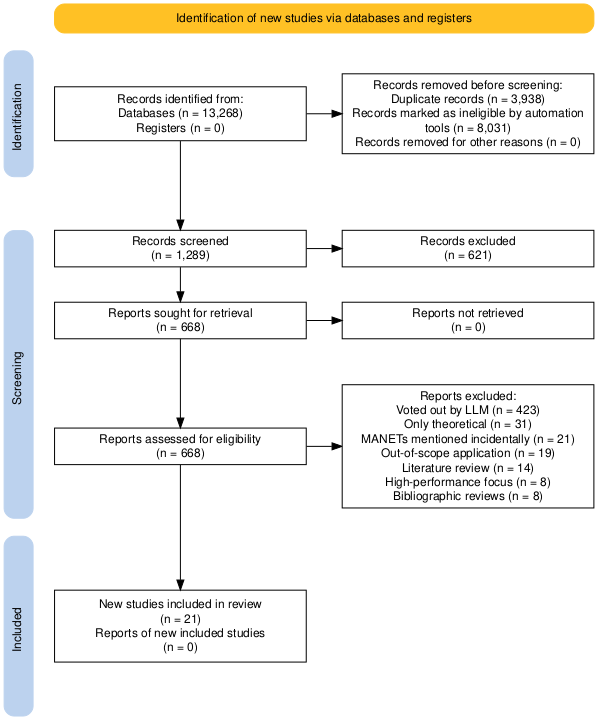
\includegraphics[width=0.7\textwidth]{./assets/prisma.png}
\caption{Диаграмма PRISMA-ScR}
\end{figure}

\subsubsection{Анализ временных рамок}\label{timeframe-analysis}

Собранные статьи охватывают временной диапазон
с 1998 по 2024 год,
хотя практически все статьи были опубликованы после 2010 года.
Максимальное количество публикаций за один
год составило три статьи --
так произошло в 2012, 2013, 2015 и 2020 годах.
Гистограмма распределения статей по годам показана на рис. \ref{pic:years}.

Это показывает,
что задачи маршрутизации в динамических меш-сетях рассматривалась
еще в конце 1990-х годов,
однако значительное развитие эта область получила
только с 2010-х годов,
когда оборудование для поддержки беспроводных
меш-сетей стало широко доступным.

\begin{figure}[p]
\centering
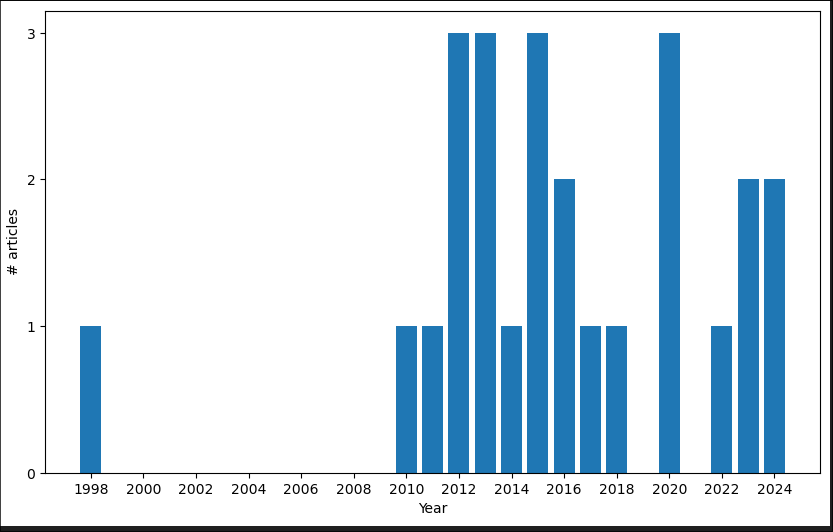
\includegraphics[width=0.7\textwidth]{./assets/by-year.png}
\caption{Распределение статей по годам}
\label{pic:years}
\end{figure}

\subsubsection{Географическое распределение публикаций}\label{geographical-distribution-of-publications}

Наибольшее количество публикаций приходится на Китай -- 7 статей.
Следующей идет Индия с 5 статьями,
затем Пакистан, Канада и Испания,
каждая из которых имеет 3 статьи.
Остальные выделенные на рис. \ref{pic:country} страны имеют по 1 статье каждая.

Для простоты подсчета учитывается только принадлежность
основного автора, однако некоторые статьи
имеют соавторов из других стран,
поэтому это не исчерпывающий список всех авторов.
Например, некоторые статьи имеют соавторов из США,
однако США на приведенном ниже рисунке не выделяется.

Эти данные подсказывают, что
меш-сети -- глобально актуальная область исследований.
Китай известен как центр мирового производства
потребительских технологических устройств,
а Индия лидирует по развитию технологий программирования,
что объясняет, почему эти страны представленны настолько сильно.

\begin{figure}[p]
\centering
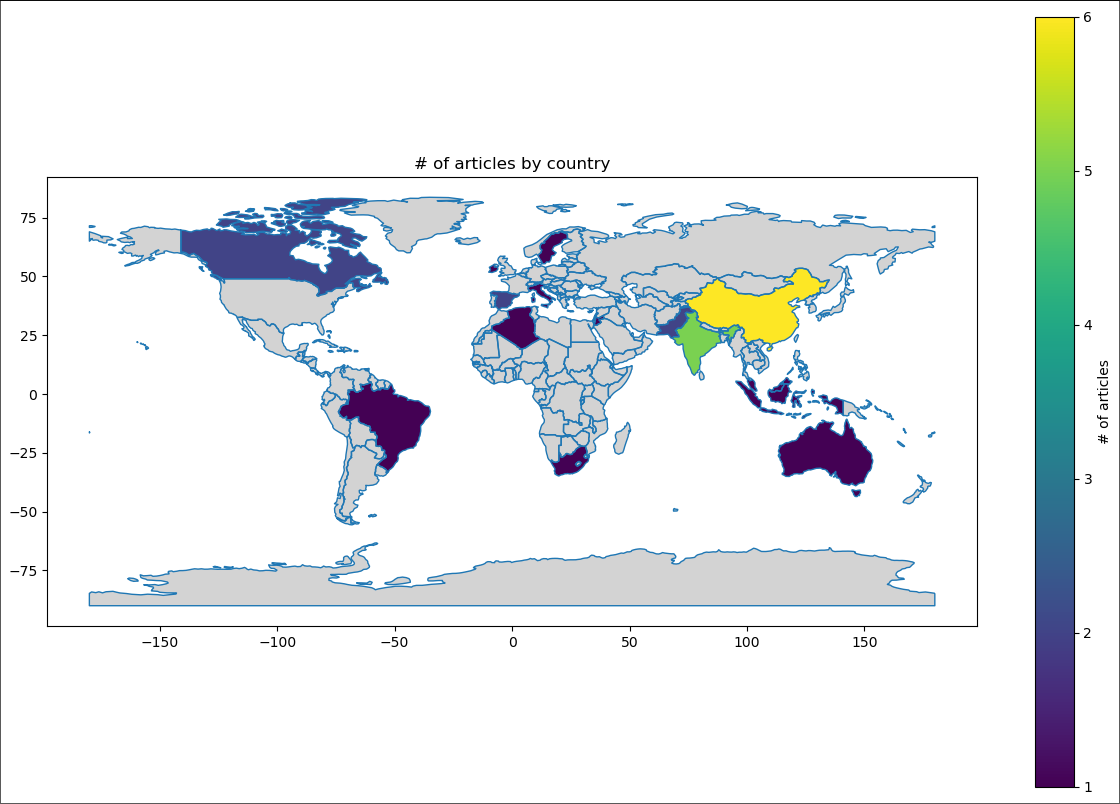
\includegraphics[width=0.7\textwidth]{./assets/by-country.png}
\caption{Распределение статей по странам}
\label{pic:country}
\end{figure}

\section{Определение текущих трендов}\label{defining-current-trends}

\begin{figure}[p]
\centering
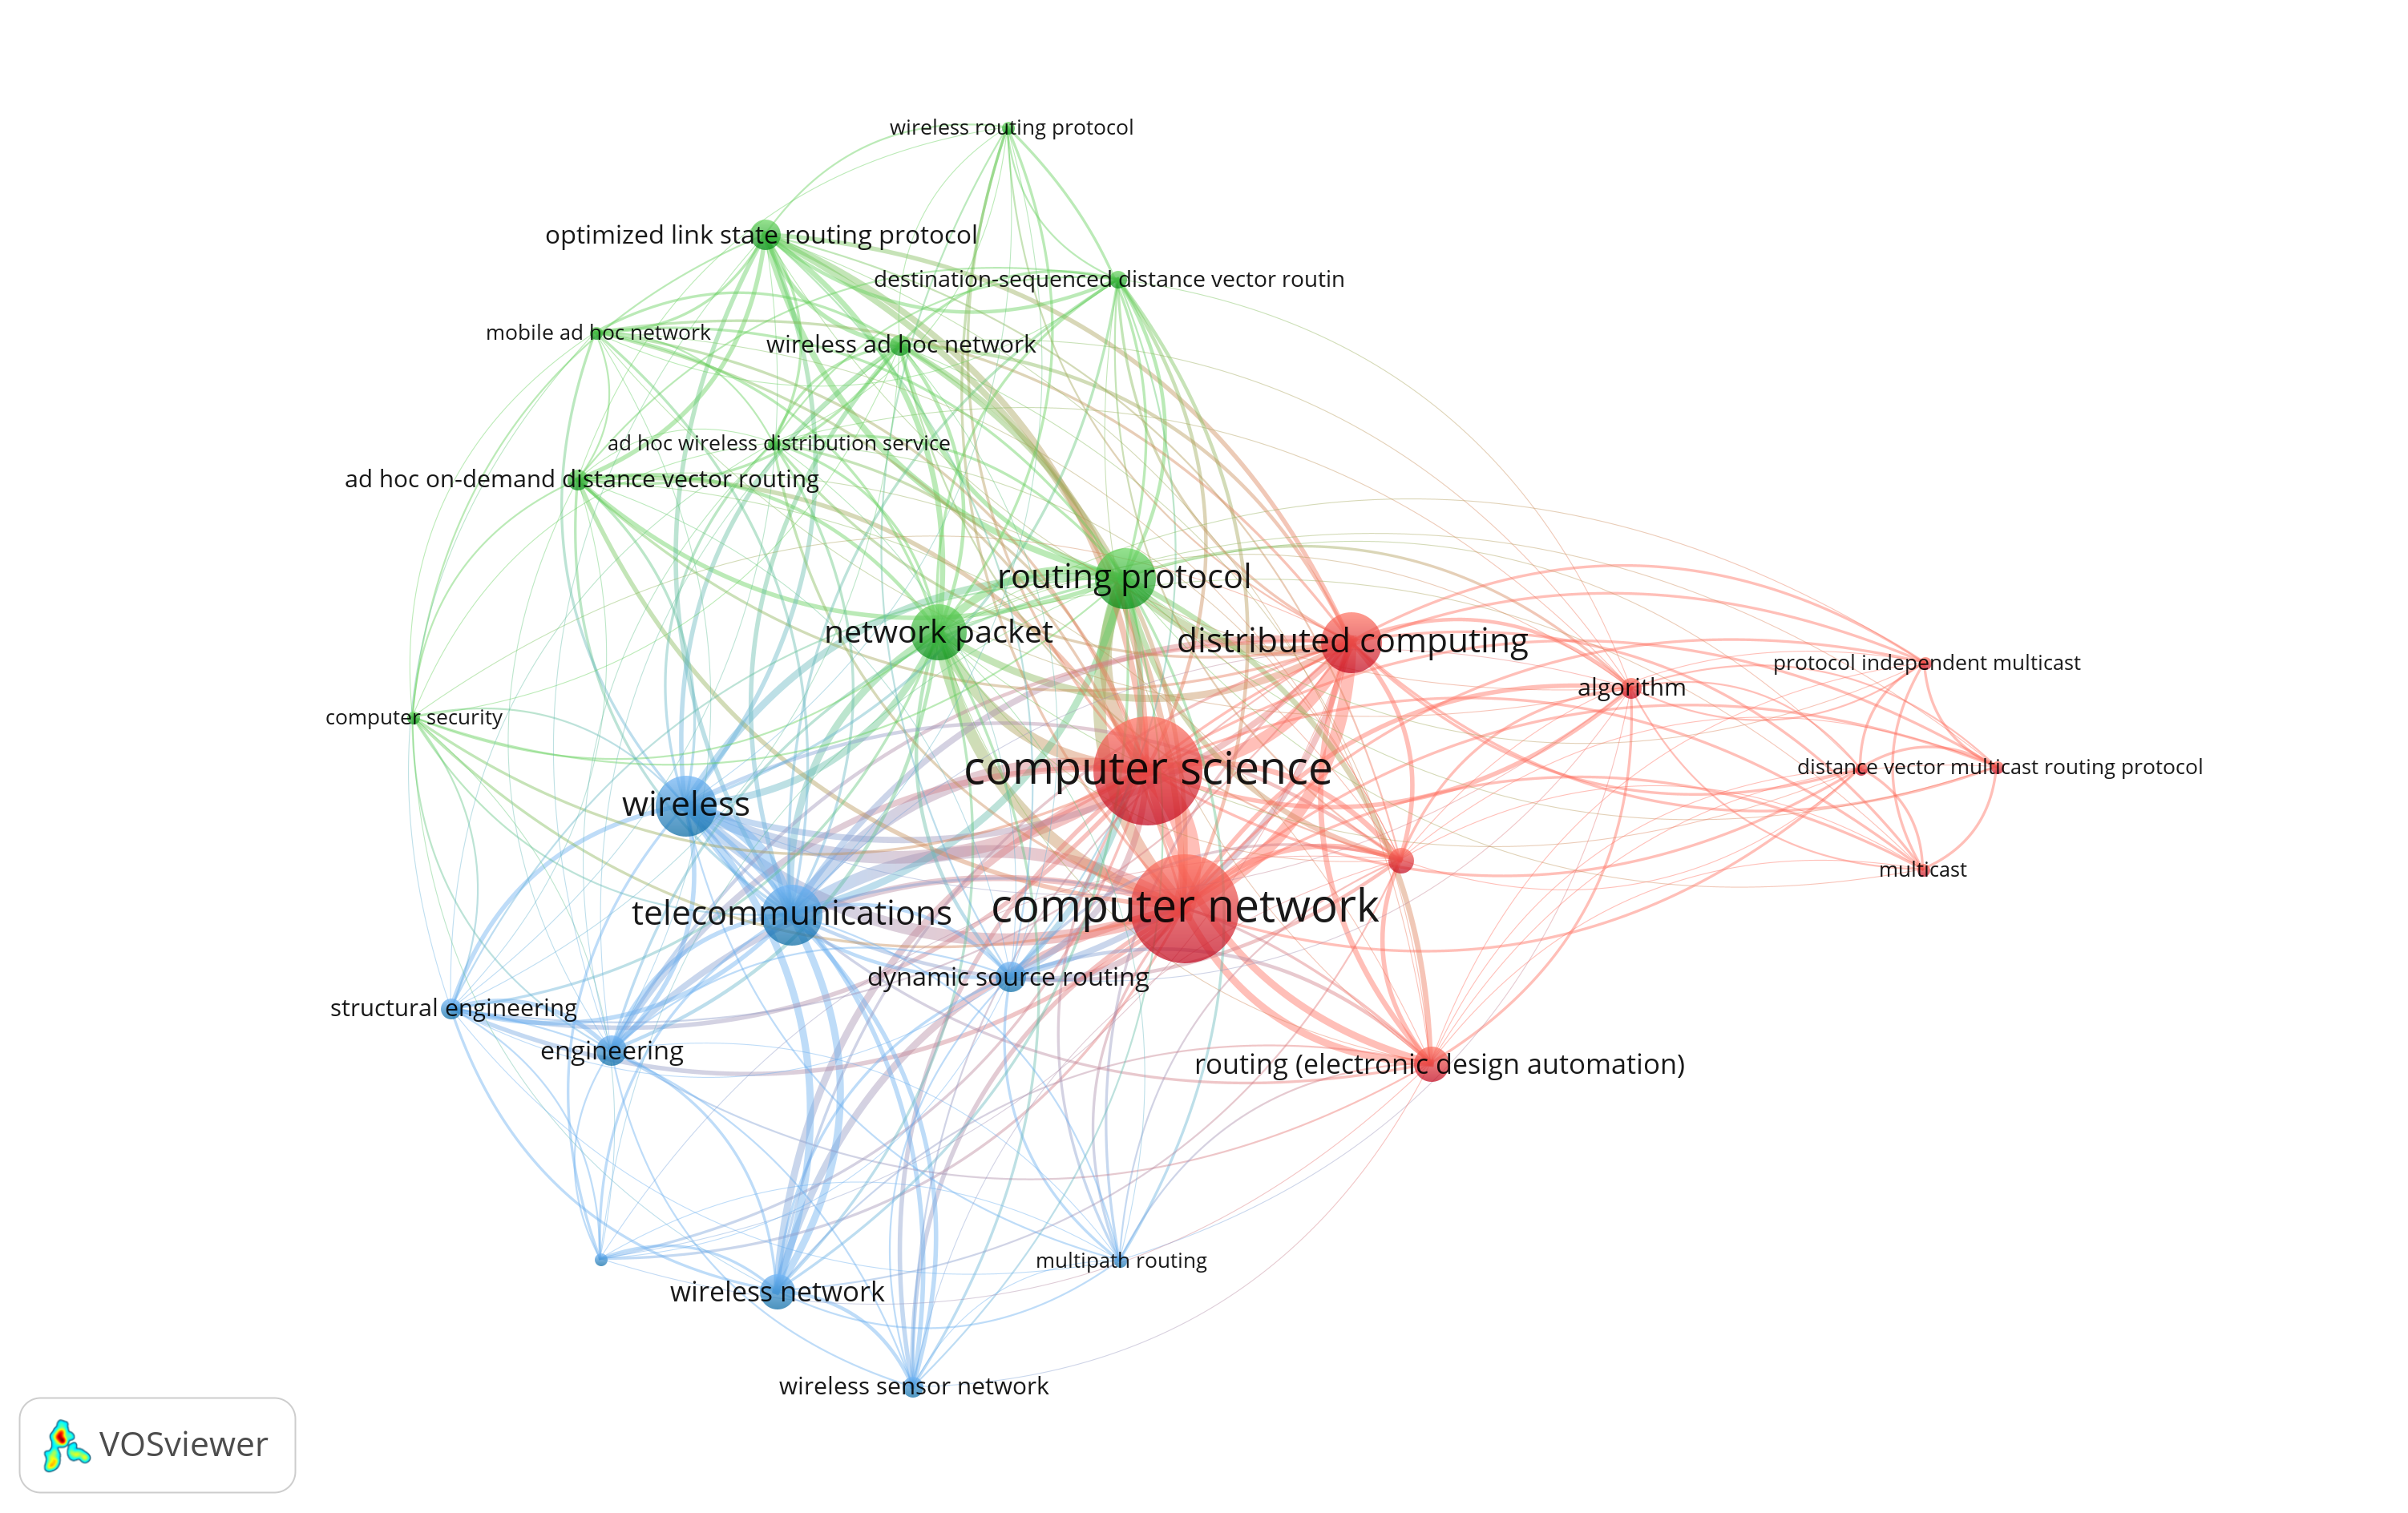
\includegraphics[width=\textwidth]{./assets/co-occurence.png}
\caption{Карта совпадения ключевых слов}
\label{pic:vosviewer}
\end{figure}

Используя приложение VOSviewer~\cite{vanEck2010}
для анализа ключевых слов в статьях,
создан рис. \ref{pic:vosviewer} -- 
диаграмму, на которой показаны ключевые слова,
и сила соединений между ними показывает то,
насколько часто они встречаются вместе.
На этой диаграмме можно найти
три основных кластера:

\textbf{Информатика:} Этот кластер (показанный красным)
связан с теоретическими основами информатики,
в том числе алгоритмами
(в особенности в <<distributed computing>> -- распределенных вычислениях -- 
которая является центральным элементом).
Некоторые ключевые слова,
связанные с сетями (такие как <<multicast>>),
также находятся здесь,
потому что они лежат в основе
многих теорий разработки алгоритмов.

\textbf{Маршрутизация:} Этот кластер (показанный зеленым)
имеет акцент на конкретной задаче
передачи сетевых пакетов -- 
<<network packets>> -- с помощью протокола маршрутизации -- <<routing protocol>>,
например <<optimized link state routing protocol>>.
Конкретно этот протокол является популярным выбором для
беспроводных меш-сетей,
поэтому есть довольно сильная связь с <<wireless ad-hoc network>>.

\textbf{Телекоммуникации:} Этот кластер (показанный синим)
исследует с конкретные проблемы,
связанные с подключением компьютерных систем друг к другу.
Здесь можно найти ключевое слово <<wireless>> -- <<беспроводной>> -- 
которое в других кластерах всегда является частью другого слова. 
Кроме того, здесь появляется слово <<engineering>>,
и в частности <<structural engineering>> -- (строительное) инженерное дело --
потому что здесь есть упор физический дизайн зданий,
который имеет особое значение для эффективного распространения
беспроводных радио-сигналов.

Эти три кластера тесно связаны вместе,
потому что (для примера)
невозможно провести четкое разделение между
маршрутизацией в частности и телекоммуникациями в общем.
Из-за этого есть сильные связи между понятиями
<<wireless>>, <<routing protocol>>, <<telecommunications>> и
<<network packet>> (<<беспроводной>>, <<протокол маршрутизации>>, <<телекоммуникации>>
и <<сетевой пакет>>):
каждое из этих понятий имеет отражение в других,
поэтому их нельзя четко разделить.
Аналогично, хотя
<<distributed computing>> (распределенные вычисления)
имеет самую сильную связь с <<computer
science>> и <<computer network>> (<<информатика>>, <<компьютерная сеть>>),
также существует весьма сильная связь с 
<<network packet>> (сетевой пакет),
потому что в распределенных вычислениях
часто требуется хорошее понимание того,
как работает физическая инфраструктура маршрутизации пакетов,
на которую опирается приложение.

Наконец, понятия вроде  <<engineering>> (инженерное дело)
не являются центральными в диаграмме,
но тем не менее важны,
и это подчеркивает тот факт, 
что теоретические основы меш-сетей
все-таки используются в практических задачах.

%\subsection{Синтез результатов}\label{synthesis-of-results-1}

\subsection{Используемые методы}\label{methodology-details}

\subsubsection{IoT-оборудование}\label{iot-hardware}

Во многих исследованиях идет речь про использование
беспроводных сенсорных устройств
и встраиваемых систем с низким энергопотреблением,
которые используют общепринятые стандарты для коммуникации,
например IEEE 802.15.4 и IEEE 802.11.

В работе \textcite{KRENTZ202457}
используются устройства на базе стандарта IEEE 802.15.4,
известного своей пригодностью для
сред с низким энергопотреблением и низкой
скоростью передачи данных -- в потребительском сегменте
он называется ZigBee и часто рекламируется
в контексте низкомощных IoT-устройств,
например работающих от аккумуляторов.
Напротив, \textcite{SAIF2015404,KABIWA20131108}
используют MAC-уровень,
предоставляемый IEEE 802.11 (более известный как Wi-Fi),
который работает с более высоким энергопотреблением
и более высокой скоростью передачи данных,
что подходит для более сложных устройств
вроде смартфонов и ноутбуков.

Некоторые исследования~\cite{SHARMA2013416,VENKATESHA201537}
используют мобильные и стационарные сенсорные узлы,
обычно применяемые в сценариях
экологического и промышленного мониторинга.
В некоторых работах~\cite{HECK2025110364,HASAN2018454}
рассматриваются умные счетчики для энергосетей,
которые передают показания использования энергии
постоянно,
что отражает растущую интеграцию IoT
в энергетическую инфраструктуру.

Исследования, основанные на моделировании,
такие как \textcite{DIIANNI1998131,LI2011458,LIU201321},
не зависят от конкретной реализации физических аспектов
устройства,
а вместо этого моделируют узлы меш-сети
с возможностями,
характерными для реальных IoT-устройств.
В других работах~\cite{CHARLES20201819},
моделируются конкретные
реальные устройства IoT
(например, Tmote Sky motes) в симуляторах вроде Contiki Cooja,
что позволяет сосредоточиться на стандартизированных,
коммерчески доступных, аппаратных платформах.

Общей чертой этих исследований является использование
устройств с низким энергопотреблением,
беспроводной связью на коротких расстояниях
и пригодностью для работы в условиях,
когда требуется большое количество узлов,
и поэтому ввиду экономических соображений
вычислительные ресурсы ограничены
(например, промышленные объекты,
интеллектуальные электросети,
экологический мониторинг).
Это подчеркивает, что есть общепринятое понимание
аппаратных ограничений и сетевых условий,
в которых должны работать протоколы маршрутизации,
и это подтверждает актуальность стандартизированных
IoT-устройств с низким энергопотреблением в
исследовательском пространстве.


\subsubsection{Основные вопросы маршрутизации}\label{main-network-routing-considerations}

Сравнительный анализ рассмотренных статей
выявляет несколько повторяющихся вопросов,
которые возникают при разработке
и оценке протоколов маршрутизации в меш-сетях.
Чаще всего акцентируется
энергоэффективность, поддержка мобильности,
скорость стабилизации новых конфигураций,
масштабируемость сети
и вопросы безопасности.

Энергоэффективность -- одна из самых важных проблем,
которые поднимаются авторами
(и это неудивительно,
потому что именно такие условия
являются основным фокусом данного обзора).
В \textcite{KRENTZ202457}
подчеркивается необходимость минимизации
энергопотребления для продления срока жизни сети,
определяемого как время работы узлов-маршрутизаторов
от одного заряда батареи.
Эти исследования фокусируются на минимизации
повторных передач, сокращении накладных расходов
на обслуживание маршрутов и выборе маршрутов
с учетом энергопотребления.

Поддержка мобильности является еще одним
критически важным аспектом в динамических средах,
где узлы могут перемещаться -- это будет влиять на
стабильность маршрутов.
Это подробно обсуждается в \textcite{SHARMA2013416},
где представлены адаптации с учетом
мобильности и механизмы восстановления
для поддержания надежной связи при перемещении узлов.
Это связано со скоростью сходимости и стабильностью,
которые подчеркиваются например в \textcite{LI2020570},
где быстрое обнаружение маршрутов
и адаптация необходимы для поддержки
приложений реального времени и минимизации потерь пакетов.
Это важно для этой работы,
потому что в ней рассматриваются именно мобильные роботы,
которые будут менять свою конфигурацию сети
по мере движения и решения своей задачи.

Масштабируемость механизмов маршрутизации
является еще одной общей темой,
особенно в крупных или плотных сетях
(например, в беспроводных сенсорных сетях,
которые могут иметь десятки узлов в одной комнате
и тысячи по всему зданию).
В \textcite{ALVAREZ2008240}
акцентируются иерархические структуры
и межслойные протоколы как методы обработки
увеличенных накладных расходов на маршрутизацию
без ущерба для производительности.

Вопросы безопасности и конфиденциальности
рассматриваются в протоколах, таких как SMOR,
представленном в \textcite{KRENTZ202457},
где безопасная многопутевая маршрутизация
противодействует рискам подделки данных и прослушивания.
Обеспечение безопасного обнаружения маршрутов
и передачи данных особенно подчеркивается в сценариях,
связанных с конфиденциальными или критически важными данными;
однако это упомянается не во всех рассмотренных статьях,
потому что меш-сети чаще всего используются
в сравнительно доверенных контекстах (например,
как часть умного дома в одной квартире).

Такой общий фокус на энергоэффективности,
поддержки мобильных узлов, быстрой сходимости
и масштабируемости отражает
общий набор приоритетов,
которые присутствуют при дизайне протоколов
маршрутизации в беспроводных меш-сетях.


\subsubsection{Исследуемые алгоритмы}\label{used-algorithms}

Обсуждаемые в рассмотренных статьях алгоритмы демонстрируют
широкий спектр применений, но большинство из них адаптированы
к конкретным задачам использования меш-сетей.
Особое внимание уделяется оптимизации
маршрутизации, особенно с учетом требований безопасности,
энергоэффективности и динамических изменений топологии.

Например, протокол Sorting Ant,
представленный в работе \textcite{LI2020570},
разработан специально для статических меш-сетей
для создания отказоустойчивой сети в
умных сетях электроснабжения.
Аналогично, \textcite{PAN2012952}
ориентируются на меш-сети с акцентом на
поддержку многоадресной рассылки (multicast)
и динамических топологий.

Другим важным направлением являются LLN-сети
(\emph{low power and lossy network},
сеть с низкой энергией и потерями пакетов)
и беспроводные сенсорные сети (WSN),
часто развертываемые для экологического мониторинга
или городской инфраструктуры.
Алгоритм в работе \textcite{KRENTZ202457}
фокусируется на LLN в системах промышленной автоматизации,
где безопасность совмещается с  энергоэффективной
многопутевой маршрутизацией.

На другом конце спектра находятся сети
с высокой мобильностью, требующие иных подходов,
и алгоритмы вроде AODV и их улучшения~\cite{LIU201321}
хорошо подходят для таких случаев.
Приложения для умных городов и коммунальных служб
часто встречаются, особенно в алгоритмах,
разработанных для Wi-SUN FAN (\emph{field area network},
сеть с масштабами поля: наружная сеть большого размера,
например соединяющая вместе городские фонари)
и Bluetooth Low Energy (BLE) меш-сетей.

Механизм Fast Routing Recovery (FRR),
предложенный в работе \textcite{HECK2025110364},
адаптирован для сетей Wi-SUN FAN,
используемых в интеллектуальном учете электричества,
где минимизация потерь пакетов важна для
надежной передачи данных в реальном времени,
но при нарушениях разрешается передать эту информацию позднее.
Аналогично, \textcite{HERNANDEZSOLANA2022109114},
фокусируются на BLE Mesh сетях,
оптимизируя энергосбережение и устойчивость к задержкам
в IoT-сетях.

Общие темы во всех статьях включают
адаптацию протоколов маршрутизации к
физическим и специфическим для приложений
ограничениям сети, таким как мобильность узлов,
доступность питания и необходимость безопасной
коммуникации. Большинство алгоритмов адаптированы
для статических или полустатических развертываний,
хотя растет внимание к мобильным сетяи и системам низкой задержки,
особенно в WSN и меш-топологиях.

В статьях, таких как \textcite{LI2011458},
показано, что стратегии, использующие многопутевую
и многоканальную маршрутизацию, предпочтительны для
повышения надежности и пропускной способности в таких сетях.
Ключевой вывод заключается в том, что ни
одна из перечисленных статей не использует
традиционные алгоритмы маршрутизации вроде
BGP, RIP или OSPF (которые являются стандартными
протоколами для статических IP-сетей,
составляющих Интернет). Вместо этого специфические
ограничения задачи побуждают авторов разрабатывать
новые алгоритмы, адаптированные к потребностям
конкретной области.

\subsection{Методы оценки результатов}\label{measuring-outcomes}

\subsubsection{Симуляторное программное обеспечение}\label{simulator-software}

Компьютерное моделирование было преобладающим
методом оценки во всех статьях. Многие
исследования использовали сетевой симулятор
Cooja вместе с операционной системой Contiki-NG~\cite{HECK2025110364,KRENTZ202457}.
В работе \textcite{SHARMA2013416} проводилось
моделирование с 40 мобильными узлами в среде
площадью 100 кв.метров для оценки
надежности динамической маршрутизации.

NS2 и NS3 также использовались в
нескольких исследованиях для моделирования
статических mesh-топологий и оценки скорости
сходимости. Некоторые авторы предпочли разработать
собственное программное обеспечение сетевого симулятора
для своей задачи~\cite{PAN2012952}.
Это может быть полезно для быстрого прототипирования,
но ограничивает возможности воспроизводимости и сопоставимости
результатов.

Среди менее используемых симуляторов был TOSSIM
(симулятор для приложений TinyOS -- это встроенная операционная
система для приложений с низким энергопотреблением),
который использовался в работе
\textcite{KAFI2014181}.
В работе \textcite{ALVAREZ2008240}
отсутствовало специальное программное обеспечение
для моделирования, однако были представлены
как теоретические, так и основанные
на моделировании стратегии оценки.

Такой разнообразный подход к выбору инструментов
симуляции отражает специфику исследуемых задач и
подчеркивает важность правильного выбора инструментария
для оценки протоколов маршрутизации в различных
условиях и сценариях применения.

\subsubsection{Практическое тестирование}\label{field-testing}

Ни одно из включенных исследований
не сообщало о масштабных полевых испытаниях
в реальных условиях; вместо этого они опирались
на среды моделирования для воспроизведения условий реального мира.
Однако параметры моделирования часто тщательно
подбирались для приближения к реалистичным сценариям --
например, в симуляции воспроизводилась
городская планировка
или траектории движения мобильных узлов.
В одном исследовании~\cite{VENKATESHA201537},
даже были выбраны конкретные бюджеты энергии
и энергетическая стоимость отправки радиосообщений
(конкретно, каждый узел имел запас 5 Дж в батарее
и тратил 0.0255 Дж на передачу).
В другой работе~\cite{KRISHNA2016817}
в окончательных результатах приводятся показатели
эффективности работы радиомодулей в джоулях.

Только одно исследование,
\textcite{MUHENDRA2017332},
выполняло какие-либо полевые испытания на оборудовании,
используя небольшое самодельное устройство,
состоящее из микроконтроллера ATmega328p
и WiFi-модуля ESP8266.
Такое устройство может быть компонентом
IoT-решения, например для умного дома,
поэтому тот факт, что меш-сеть функционировала
(с допустимой производительностью, например
средняя скорость передачи данных составляла 110 кбит/с),
означает, что возможно развернуть такие
тесты с использованием стандартного оборудования.

\subsubsection{Особенности алгоритмов в зависимости от задачи}\label{specific-considerations-for-algorithm-usage-scope}

Каждый алгоритм был адаптирован под конкретный
профиль ограничений.
Например, SMOR оптимизирован для LLN-сетей, что
делает его подходящим для приложений
умного дома или удаленного мониторинга.
FRR специально разработан для сетей Wi-SUN FAN,
актуальных в инфраструктуре интеллектуальных электросетей.
Алгоритм FNA-CTP предназначен для высокомобильных WSN,
особенно в транспортных или аварийно-спасательных контекстах.
Протокол Fortified Ant ориентирован на мобильные меш-сети,
делая акцент на безопасной многопутевой маршрутизации,
подходящей для полустатических сетей.
Между тем, многоуровневый подход в работе
\textcite{ALVAREZ2008240}
разработан для статических сенсорных сетей,
в частности в сборе экологических данных.

Поскольку энергия является дефицитным ресурсом,
некоторые алгоритмы предусматривают несколько классов узлов.
Например, в работе \textcite{ZHENG2020443},
(где развернута беспроводная сенсорная сеть)
существуют сенсорные узлы (Sensor Nodes),
которые только собирают и отправляют данные,
кластерные узлы (Cluster Nodes),
формирующие основную ткань сети,
и главы кластеров (Cluster Heads),
хранящие информацию о маршрутизации,
которые избираются в зависимости от того,
сколько у них энергии в батарее.
Аналогично, в работе \textcite{LI2020570}
обычный <<протокол колонии муравьев>>
усовершенствован до Fortified Ant
с добавлением так называемых <<элитных муравьев,>>
которые оказывают большее влияние на маршрутизацию,
чем соседние узлы (согласно алгоритму, они <<выпускают больше феромонов,>> чем другие муравьи).
Такое разделение узлов позволяет более простым
и менее мощным узлам заботиться только о
собственных данных,
оставляя задачу маршрутизации данных
более мощным узлам.
(Некоторые статьи,
такие как \textcite{ALI2024102356},
фактически в первую очередь сосредоточены на этапе голосования,
поскольку улучшения в избирательном процессе узлов-лидеров
приводят к улучшению качества маршрутизации во всей сети.)

Теоретический подход, описанный в работе
\textcite{DIIANNI1998131}, возможно, является самым гибким
из всех рассмотренных статей, поскольку он применим к
любой пакетной сети -- проводной или беспроводной -- и
статья сосредоточена на ограничениях по задержке
и пропускной способности, которые неизменно
присутствуют во всех реальных сетях.
Однако вывод этой статьи заключается в том,
что обобщенная задача пакетной маршрутизации не может быть
эффективно решена за полиномиальное время
(т.е. это задача класса NP).
Это означает, что в реальных развертываниях меш-сетей
приходится жертвовать либо временем передачи
пакетов от одного узла до другого,
либо пропускной способностью,
либо энергоэффективностью,
и все остальные статьи так или иначе справляются
с этим ограничением.

Таким образом, несмотря на разнообразие подходов
и специализацию алгоритмов под конкретные задачи,
все они сталкиваются с фундаментальными ограничениями
в эффективности маршрутизации и вынуждены находить
компромиссы между различными параметрами сети.

\subsubsection{Измеряемые метрики и цели}\label{evaluation-metrics-and-targets}


В рассмотренных исследованиях использовался
ряд симуляционных сред и метрик производительности
для оценки эффективности алгоритмов маршрутизации в меш-сетях.
Среди часто используемых инструментов моделирования:
NS-2, NS-3, Cooja с операционной системой Contiki-NG,
а также самописные симуляторы,
часто моделирующие статические топологии или
мобильные топологии с рандомизированными схемами движения.
Метрики, используемые для оценки производительности,
демонстрируют согласованность в литературе:
особое внимание уделяется показателям вроде
PDR (\emph{packet delivery ratio}, вероятность доставки пакетов),
end-to-end latency (задержка от отправки пакета одним узлом до получения его другим),
энергопотребление,
процент трафика, связанный с внутренними аспектами работы сети,
и время сходимости сети после изменений топологии.

В работе \textcite{KRENTZ202457} продемонстрирована
комплексная оценка с использованием
Cooja и Contiki-NG в динамических и статических условиях сети.
Были выделены такие метрики, как PDR,
задержка, энергопотребление и объем памяти.
Предложенный алгоритм SMOR достиг значительных
улучшений в надежности и времени доставки сообщений,
обладая при этом высокой отказоустойчивостью и усилением
безопасности (таким как устойчивость
к поддельным узлам и DoS-атакам).

\textcite{HECK2025110364} симулируют сеть в
Cooja и измеряют время формирования сети
и энергоэффективность, достигая ускорения восстановления
до 50\% после
перезагрузки сети,
при этом сохраняя низкое время активности радио.

Некоторые статьи больше обращают внимание на метрики
пропускной способности и задержки,
используя многопутевые (\emph{multipath})-стратегии для минимизации
задержки при multicast-рассылке и для повышения
пропускной способности~\cite{KUMAR2012481,LI2011458}.

Энергоэффективность также выделяется как важное
преимущество во многих исследованиях. Например,
\textcite{HERNANDEZSOLANA2022109114} сообщает
о экономии энергии до 99,24\% по результатам
симуляции, что достигается за счет
того, что радиомодуль больше времени проводит в выключенном состоянии.

В работе \textcite{PAN2012952} подчеркиваются
улучшения как PDR, так и задержки,
особенно в сценариях с мультимедийным трафиком.
Другие исследования либо дают теоретическую оценку,
либо качественный анализ,
но почти все подчеркивают такие преимущества,
как простота архитектуры и сокращение задержек~\cite{ALVAREZ2008240,DIIANNI1998131}.

Таким образом, несмотря на разнообразие подходов
оценки, многие статьи сообщают похожие метрики,
что позволяет делать некоторые сравнения
эффективности различных алгоритмов
маршрутизации.

Несмотря на различия в тестовых стендах и протоколах, можно выделить некоторые четкие закономерности:

\begin{itemize}
\item    Вероятность доставки пакетов (PDR)
является наиболее сообщаемой метрикой,
часто связанной с утверждениями об улучшении надежности.
\item  Задержка доставки пакетов
и время сходимости сети обычно
используются для оценки быстродействия и адаптивности.
\item    Энергопотребление доминирует
как метрика в исследованиях,
ориентированных на датчики и IoT,
особенно в крупных или ресурсоограниченных сетях.
\item    Нагрузка на поддержание сети
используется для оценки эффективности, особенно в протоколах
с реактивным или гибридным дизайном.
\item    Платформы моделирования
(NS2, NS3, Cooja, TOSSIM) предпочитают из-за их
гибкости, и очень немногие исследования включают
тестирование в реальных условиях.
\end{itemize}

Во всех рассмотренных статьях предложенные
алгоритмы демонстрируют
преимущества с точки зрения надежности,
эффективности и масштабируемости ---
часто за счет многопутевой маршрутизации,
пересылки пакетов с вероятностными подходами
и стратегий, учитывающих мобильность.
Большинство из
рассмотренных улучшений имеют инкрементальный характер,
потому что они основаны на существующих протоколах
(таких как RPL, AODV или CTP)
с усовершенствованиями, адаптированными под конкретные сценарии,
например для улучшения мобильности,
энергосбережения или быстроты восстановления.

\section{Обсуждение}\label{discussion}

\subsection{Обобщение результатов}\label{summary-of-evidence}

В рассмотренной литературе подчеркивается важность
аппаратных платформ низкого энергопотребления в
исследованиях маршрутизации в меш-сетях,
особенно платформ, которые соответствуют стандартам вроде
IEEE 802.15.4 и IEEE 802.11.
Эти платформы -- как универсальные коммерческие устройства,
так и сенсорные узлы, специально разработанные для конкретных исследований --
отражают ограниченные возможности по энергопотреблению,
пропускной способности и обработке данных,
типичные для IoT.
Для моделирования реальных сетевых условий обычно
используются симуляторы,
такие как Cooja и NS2/NS3, которые позволяют настраивать
баланс между экспериментальным контролем и реализмом.

Проектирование протоколов маршрутизации
во всех рассмотренных статьях формируется
вокруг общего набора приоритетов --
энергоэффективность, поддержка мобильности,
масштабируемость и быстрое время сходимости.
Энергоэффективность выделяется как ключевая проблема
из-за ограниченного времени работы батарей
сенсорных узлов; чем более эффективно используется радио-модуль,
тем реже нужно вручную менять батарею,
и тем больше сенсоров можно обслуживать одним и тем же количеством персонала.
Многие работы предлагают
методы маршрутизации, которые минимизируют
повторные передачи, сокращают затраты на
обслуживание маршрутов и используют метрики выбора
пути с учетом энергопотребления.

Поддержка мобильности также имеет важное значение,
особенно в сценариях, где узлы могут перемещаться 
(особенно когда это движение не контролируется сетью:
в случаях мобильных роботов сеть может подготовиться к тому,
что какой-то узел выйдет за радиус действия).
Протоколы, которые быстро адаптируются к изменениям в
топологии сети или включают механизмы восстановления,
демонстрируют хорошую надежность в условиях мобильности.

Хотя алгоритмы маршрутизации различаются по
структуре и направленности, все они адаптированы
под конкретные потребности предполагаемых приложений.
Примеры таких протоколов, как SMOR, FRR и Fortified Ant,
решают задачи в LLN, Wi-SUN FAN или меш-сетях
соответственно. Некоторые протоколы используют
иерархические или ролевые подходы --
такие как выбор головных узлов кластера или
элитные модели муравьев: это позволяет им
распределять нагрузку (и энергопотребление)
только на те узлы, которые способны в данный момент
выдержать ее.
Примечательно, что ни один из рассмотренных алгоритмов
не опирается на традиционные интернет-протоколы маршрутизации
вроде BGP или OSPF. Вместо этого они
используют специальные методы, которые лучше соответствуют
динамической и децентрализованной природе меш- и сенсорных сетей.

Моделирование остается основным методом оценки
производительности протоколов. Широко используются инструменты вроде Cooja, NS2/NS3 и TOSSIM,
хотя некоторые исследования также применяют
симуляторы, разработанные ими самостоятельно. Общие показатели
производительности включают процент доставляемых пакетов, задержку доставки,
энергопотребление и служебную нагрузку на поддержание сети.
Большинство работ сообщают об улучшениях по сравнению
с существующими базовыми протоколами.

Поскольку различные стратегии маршрутизации
нацелены на разные варианты использования IoT,
каждое исследование обычно фокусируется
на определенном наборе метрик: некоторые
отдают приоритет PDR, другие подчеркивают
время сходимости сети, а третьи
стремятся снизить энергопотребление за
счет снижения пропускной способности данных.
Хотя тестирование на аппаратном
обеспечении встречается редко, симуляции
часто настраиваются с реалистичными параметрами
батарей и энергопотребления для более точного
отражения реальных условий.

В общем, в литературе наблюдается четкая
тенденция в работах с  меш-сетями:
протоколы маршрутизации становятся более адаптивными,
легковесными и ориентированными на определенный контекст,
и они формируются под влиянием конкретных
потребностей IoT-систем. Хотя многие
из предложенных решений строятся на
основе существующих работ,
они вносят улучшения в надежность,
эффективность и масштабируемость для энергоограниченных
динамических сетей. Область по-прежнему в
значительной степени ориентирована на симуляцию,
и в будущем есть возможности
для стандартизации методов оценки и расширении
тестирования на реальном оборудовании.

\subsection{Ограничения}\label{limitations}

Можно определить некоторые ограничения в существующем спектре
исследований.

\subsubsection{Отсутствие стандартов оценивания эффективности}\label{lack-of-uniform-evaluation-standards}

Отсутствие единых метрик оценки в различных исследованиях
создает проблему для проведения содержательных сравнений.
В одной статье важнейшей метрикой является PDR,
а в следующей -- время сходимости сети
(при этом потеря пакетов считается допустимой):
при оптимизации этих двух различных факторов
сложно сравнить производительность двух сетей,
и практически невозможно сделать это на основе данных,
содержащихся в самих статьях,
так как между двумя наборами метрик существует мало пересечений.

Чтобы сравнить метрики, более специфичные для
конкретного приложения, потребовалось бы запустить
симуляции параллельно, но это затрудняется тем фактом,
что разные авторы выбрали различные симуляторы для своего моделирования.
Это создает существенные препятствия для
объективного сравнения результатов различных работ.
В результате сложно сделать обоснованные выводы
о преимуществах или недостатках различных подходов,
что затрудняет прогресс в области и разработку
более эффективных решений.

Для решения этих проблем
следует разрабатывать код для единого интерфейса,
который можно было бы запускать на различных симуляторах.
Также следует придумать стандартные задачи
и метрики, чтобы
разные авторы могли бы запустить свой код
над этими стандартными задачами и сравнить результаты напрямую.

\subsubsection{Зависимость от результатов симуляций}\label{dependence-on-simulation-based-evidence}

Значительная часть результатов в
рассмотренных работах основана на симуляциях,
а не на реальных внедрениях или полевых тестированиях.
Хотя симуляции предоставляют возможность контролируемого
тестирования, они могут не полностью отражать
сложности развертывания беспроводных меш-сетей в
реальных условиях. В частности,
беспроводные сигналы в нелицензированных радиодиапазонах
часто подвергаются помехам от других устройств,
и сложно смоделировать это в программном обеспечении иначе,
чем просто отбрасывая пакеты.
Реальные сигналы помех могут быть ошибочно приняты
за настоящие пакеты,
поэтому любое тестирование радио-протоколов
нельзя считать полноценным без того, чтобы проверить
поведение радио-системы в шумном окружении в реальном мире.

Преодоление этих ограничений
в будущих исследованиях может быть
достигнуто за счет более широких критериев включения,
стандартизированных метрик и интеграции реальных кейсов.
Это позволит повысить всесторонность и актуальность обзора.


\chapter{Разработка симулятора} 
\label{sec:base-section}

В рамках обзора литературы найденно несколько существующих приложений,
которые часто используются для изучения работы меш-сетей.
Некоторые из симуляторов помогают с моделированием конкретных аппаратных платформ:
например, Cooja -- симулятор,
который позволяет запускать код на базе Contiki-NG~\cite{Contiki-NG}:
это операционная система для определенных микроконтроллеров,
предназначенная для устройств IoT.
Однако для этой задачи такие платформы не подходят,
потому что они требуют определенных аппаратных платформ,
которые часто сложно приобрести.

Другие симуляторы, например NS3,
подразумевают свой собственный интерфейс.
Приложения, написанные для этого интерфейса,
можно использовать только с этим симулятором,
и не могут быть портированны на физическое оборудование
без того чтобы переписать их с нуля.
Такие симуляторы существуют в основном,
чтобы оценить работу алгоритмов абстрактно,
на виртуальной платформе,
прежде чем реализовать ту же самую логику
заново для аппаратного интерфейса.

Симуляторы второго типа больше полезны на этапе концептуального моделирования,
когда архитектура разрабатываемой системы еще не известна.
Для практических систем больше полезны симуляторы первого типа,
потому что код для них можно напрямую прошить на физический микроконтроллер, 
но симулятор должен быть совместим с выбранной аппаратной платформой.

Из-за этого, в рамках этой работы возникла задача написать свой собственный симулятор первого типа,
который точно соответствует требованиям задачи.
Этот симулятор написан на языке Rust,
который позволяет компилировать один и тот же код
для симулятора на x86-платформе,
для микроконтроллера вроде RPi Pico,
а также для WebAssembly для испытания в веб-браузере.

\section{Беспроводное оборудование}

Одно из первых решений, которые необходимо было принять при разработке этого проекта --
какое физическое беспроводное оборудование использовать, как модель для разработки
симулятора \footnote{Результаты разработки, включая исходный код для симулятора и для этой статьи, можно найти в интернете по адресу \texttt{https://github.com/rudn-lab/planning-mesh-swarm}.}.
В этом учитывались несколько факторов:

\begin{enumerate}
\item Фрейминг: задача работы с физическими (L1 и L2 по OSI-модели) фреймами уже была решена существующими протоколами передачи данных,
поэтому модуль, который сам занимается обработкой их из радиосигнала,  который дает доступ к уже готовым кадрам или пакетам.
\item Обнаружение канального уровня (\emph{link-layer}): поскольку некоторые протоколы маршрутизации (например, OSPF и его улучшения~\cite{rfc5614}) требуют,
чтобы элементы сети могли понять, когда их соединение с соседом работает или нарушается,
хочется использовать такое оборудование, которое уже имеет такую возможность.
(Если это не существует на уровне оборудования, то можно реализовать это виртуально,
отправляя пинг-сообщения друг другу,
но это добавляет сложность в код приложения.)

\item Идентификация: чтобы в бизнес-логике не приходилось создавать и подтверждать уникальные личности для участников сети,
предпочтительно, чтобы модули имели свой собственный уникальный идентификатор (например, MAC-адрес),
и передавали его автоматически с каждым сообщением:
тогда перед нами не стоит задача отличать одного отправителя от другого. 

\item Цена: у нас ограниченные материальные ресурсы для этого проекта, поэтому модули, коорые используются для физической реализации,
должны составлять малую долю всего бюджета.
В частности, это делает непригодными модули вроде LoRa,
хотя они были бы хорошим выбором для практических реализаций.
\end{enumerate}

По всем этим причинам (а также из-за того,
что они уже были куплены для других проектов), в проекте используются Wi-Fi модули ESP-01,
которые в момент написания можно купить оптом за 90 рублей штука.
Эти модули основаны на чипе ESP8266~\cite{esp8266},
который может быть использован как модуль для другого микроконтроллера
или иметь свою собственную прошивку:
это может быть полезно для выполнения hardware offloading
некоторых из процессов поддержки меш-сети.

У каждого элемента сети (например, робота)
будет несколько таких модулей.
Один модуль будет использоваться для получения сигналов,
и он будет настроен в режиме AP (точка доступа).
Остальные модули будут в режиме STA (клиент точки доступа),
и они будут подключаться к чужим AP,
чтобы передавать им сообщения.

С точки зрения модели, это значит,
что каждое соединение имеет одностороннее направление.
Для того, чтобы два устройства настроили двухстороннее общение,
каждый из них должен иметь как минимум два модуля.
На рис.~\ref{fig:connections} показана более сложная схема из 5 устройств.

Этот подход, возможно, не практичен для настоящих встраиваемых устройств,
где одной из важных целей является минимизация количества деталей
и общей потребляемой энергии;
Wi-Fi широко известен как один из самых энергоемких радио-протоколов в потребительском сегменте.
Однако эта модель полезна для симуляции,
потому что она позволяет моделировать ситуацию,
когда одно устройство может передавать сигнал другому устройству,
но не получает от него ответов.
К тому же,
можно написать драйвер для другого стиля радиомодуля,
который будет добавлять совместимость с кодом,
написанным для выбранной абстракции:
для этого нужно будет только реализовать возможность создания (виртуальных)
соединений типа <<один к одному,>>
поведение которых соответствует требованиям модели.

\begin{figure}[p]
  \centering
  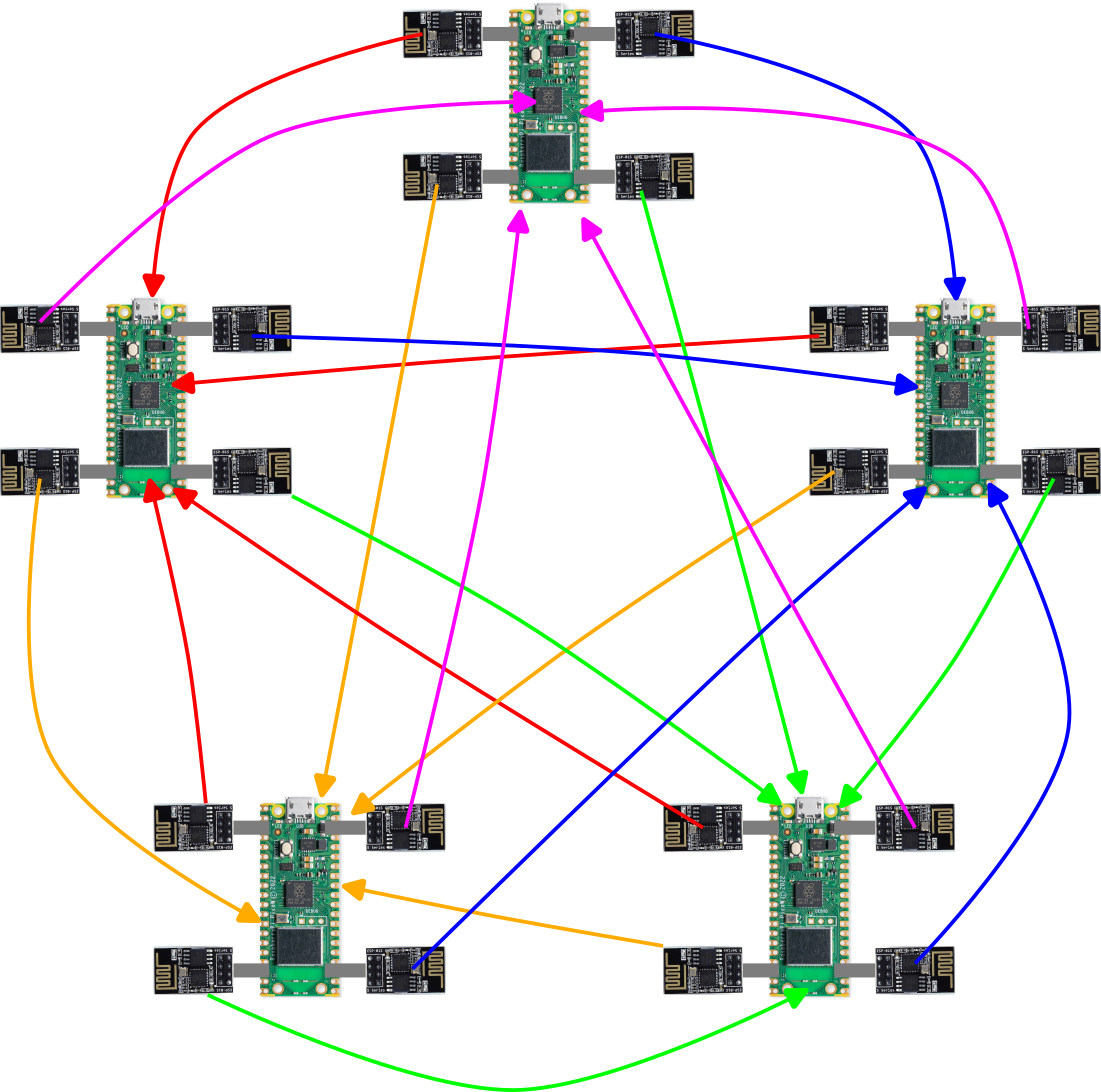
\includegraphics[width=\linewidth]{connections}
  \caption{Полносвязная mesh-сеть, состоящая из пяти контроллеров Raspberry Pi Pico W, каждый из которых имеет четыре радиомодуля ESP-01 (плюс свой собственный). Каждая стрелочка обозначает одно Wi-Fi соединение. Все ESP-01, от которых выходит стрелочка одного цвета, подключены к точке доступа, которая создается контроллером, на который указывает стрелочка. Информация двигается по направлению стрелочки.}
  \label{fig:connections}
\end{figure}


\section{Геометрия симулятора}

Этот симулятор сделан в контексте задачи мультиагентного планирования,
и для упрощения логики планнера,
обычно такие задачи имеют дело с дискретным миром.
Кроме того, при переносе этой реализации на физических роботов,
они должны понимать,
в какой точке пространства они находятся.
Из-за этого, довольно рано в процессе разработки проекта, было принято решение,
что роботы двигаются по квадратной сетке,
останавливаясь на пересечениях линий этой сетки.

С точки зрения логики движения, робот может свдинуться вперед или назад на целое количество клеток,
или повернуться влево-вправо на целое количество четвертей.
Это реализуется в физическом роботе посредством датчика линии,
который отслеживает, сколько линий проехал робот вперед
или на сколько четвертей он повернулся.

Радио-симуляция, напротив, не может работать в дискретных координатах,
потому что распространение радио-сигнала должно быть изотропным,
то есть симметричным относительно вращения~\footnote{Такая модель хорошо описывает антенны общего назначения,
например такие как в Wi-Fi модулях,
но бывают также более направленные антенны.
Этот симулятор может быть использован и с анизотропным профилем уровня сигнала;
для этого нужно описать форму этого профиля как функцию от XY.},
но в дискретных координатах невозможно нарисовать идеальную окружность.
Из-за этого симуляция радио-связи происходит отдельно,
и пока робот двигается от одной клетки к другой,
симулятор постоянно обновляет значение силы сигнала.
Каждый кадр, когда любой робот двигается,
состояние радио-системы будет обновляться,
и вне зависимости от того,
когда радио-модуль выполняет операцию,
он всегда получит свежую информацию.

Из-за этого логика внутри робота разделяется на две части: 
драйвер движения и драйвер радио-коммуникации.
Общение между этими модулями синхронизируется с помощью общей памяти (точнее, примитивов вроде каналов и семафоров, которые основаны на общей памяти),
а большую часть времени они работают независимо.
Это можно обеспечить на многоядерных микроконтроллерах,
таких как Raspberry Pi Pico/RP2040 (которая была первым выбором платформы для этого проекта),
или с использованием асинхронных подходов к программированию,
или это тривиально возможно с помощью поддержки множества процессов внутри ядра операционной системы вроде Linux.

\section{API для пользовательского кода}

Для разработки симулятора выбран язык Rust.
Он позволяет нам писать быстрый и безопасный код,
который можно компилировать на многие платформы без изменений~\cite{10.1145/2663171.2663188,klabnik2022rust}.
Благодаря этому симулятор можно запускать как нативное приложение на Linux или Windows,
или как веб-приложение через WebAssembly~\footnote{Для демонстрации,
мы скомпилировали WebAssembly-версию, которую можно запустить в браузере по адресу \texttt{https://mesh-playground.roboticlab.ru/}.}.

Такое решение также позволяет использовать один и тот же код внутри симулятора
и также на реальном оборудовании --
это потребует лишь написания драйвера для этого оборудования.
По сравнению, многие существующие подходы
для симуляционных систем
используют языки,
которые нельзя портировать на embedded-платформы без изменений;
из-за этого нужно переписать код из симулятора на embedded-платформу
(что добавляет шансы добавить ошибки)
или же использовать более мощную платформу, которая способна
исполнять код на исходном языке программирования
(например, ROS2 используется для разработки роботов,
но она основана на Linux, поэтому робот должен содержать
Linux-компьютер, чтобы использовать ROS2-модули).

Этот драйвер представлен структурой, которая реализует нужный trait (это аналог интерфейса в Rust).
Для поддержки какой-то платформы нужно лишь реализовать соответствующие асинхронные~\footnote{Для embedded-разработки
на Rust используется популярный проект Embassy~\cite{embassy}. С помощью него даже легче писать асинхронные программы
для embedded-платформ, чем синхронные. Это отличается от разработки на Arduino, например,
где ограничения платформы приводят к тому,
что код обычно пишется в синхронном стиле на C++.}
 методы для реализации функционала.

Для управления движением шасси есть возможность выбирать, какой интерфейс обозначить,
и в данный момент (как написано раньше)
робот может сдвинуться вперед/назад на несколько клеток или сделать несколько четвертей оборотов
влево-вправо.
У него также есть возможность подождать несколько секунд,
или вывести сообщение для отладки
(оно будет видно только в симуляторе).
Этот функционал вынесен в отдельную структуру
(которая называется \texttt{AsyncUtils}):
эти методы фундаментальные для выбранного асинхронного движка,
потому что на разных платформах таймеры работают по-разному,
и из-за этого нельзя использовать один и тот же метод 
в симуляторе и на Embassy без изменений.
Например, на листинге \ref{code:basic_movement} показано,
как выглядит простая реализация логики движения:
API выглядит примерно похожим на API для Turtle в Python,
но ограниченный на ортогональные повороты.
(Сам этот интерфейс есть на листинге \ref{code:chassis}.)

\begin{listing}[p]
  \caption{Простая реализация логики движения,
  которая не общается с радио-модулем,
  а просто бесконечно двигается по квадратной спирали.}
  \label{code:basic_movement}
  \begin{minted}[fontsize=\footnotesize]{rust}
pub(crate) async fn spiral(mut chassis: impl Chassis + Send + Sync) {
    let mut side_length = 1;
    loop {
        chassis.utils().log(&format!("Spiral length is: {side_length}")).await;
        chassis.forward(side_length).await;
        chassis.turn_right().await;
        side_length += 1;
        chassis.utils().sleep(Duration::from_secs(1)).await;
    }
}
  \end{minted}
\end{listing}  

\begin{listing}[p]
  \caption{Интерфейс для шасси,
  который определяет, какие движения может произвести робот.}
  \label{code:chassis}
  \begin{minted}[fontsize=\footnotesize]{rust}
pub trait Chassis {
      async fn forward(&mut self, cells: NonZeroU8);
      async fn backward(&mut self, cells: NonZeroU8);
      async fn turn_left_quarters(&mut self, quarter_turns: NonZeroU8);
      async fn turn_right_quarters(&mut self, quarter_turns: NonZeroU8);
  
      async fn turn_left(&mut self) {
          self.turn_left_quarters(NonZeroU8::new(1).unwrap()).await
      }
  
      async fn turn_right(&mut self) {
          self.turn_right_quarters(NonZeroU8::new(1).unwrap()).await
      }
  
      async fn forward_one(&mut self) {
          self.forward(NonZeroU8::new(1).unwrap()).await
      }
  
      async fn backward_one(&mut self) {
          self.backward(NonZeroU8::new(1).unwrap()).await
      }
  
      async fn turn_left_signed(&mut self, quarters: i8) {
          if quarters > 0 {
              self.turn_left_quarters(NonZeroU8::new(quarters as u8).unwrap())
                  .await
          } else {
              self.turn_right_quarters(NonZeroU8::new(-quarters as u8).unwrap())
                  .await
          }
      }
  
      async fn turn_right_signed(&mut self, quarters: i8) {
          if quarters > 0 {
              self.turn_right_quarters(NonZeroU8::new(quarters as u8).unwrap())
                  .await
          } else {
              self.turn_left_quarters(NonZeroU8::new(-quarters as u8).unwrap())
                  .await
          }
      }
  
      fn utils(&self) -> impl AsyncUtils + Send;
  }  
  \end{minted}
\end{listing}  


Для управления радио-связью нужно учитывать возможности физического радио-модуля.
В API доступны только те методы,
для которых у ESP-01 есть готовые AT-команды:
например, сканировать соседние Wi-Fi сети,
соединиться с одной из них,
отсоединяться
и измерять уровень сигнала.
Там также есть метод, чтобы отправить сообщение тому роботу,
с которым сейчас установленно соединение,
в соответствии с моделью радио-связи, описанной выше.
(Важно подчеркнуть, что это соединение не обязательно соответствует какому-либо понятию на MAC-уровне:
сообщения могут также отправляться широковещательным способом,
важно -- чтобы только один получатель обращал внимание на них,
и чтобы отправитель знал, какой это получатель.
Такую абстракцию можно реализовать поверх транспортных протоколов,
которые не поддерживают концепцию соединений напрямую).
Эти методы описаны в листинге \ref{code:traits1} и \ref{code:traits2}.

\begin{listing}
\caption{Описание интерфейса радио-ппередатчика.
Драйвер должен реализовать этот интерфейса,
чтобы быть совместимым с симулятором.}
\label{code:traits1}
\begin{minted}[fontsize=\footnotesize]{rust}
/// Интерфейс передатчика. Он может отправлять сообщения к одному другому приемнику,
/// но он должен сначала быть соединен с ним.
/// (Wi-Fi STA, подключенный к AP).
pub trait TransmitterNic<PeerId, MessageType> {
    type Error: core::fmt::Debug;

    /// Проверяет, что данный передатчик функционирует.
    async fn ping(&mut self) -> Result<(), Self::Error>;

    /// Получает, к какому приемнику мы подключены.
    async fn get_peer(&mut self) -> Result<Option<PeerId>, Self::Error>;

    /// Получает уровень сигнала текущего подключения.
    /// Уровень сигнала может быть 0, если мы сейчас не в области
    /// доступности приемника.
    async fn get_connection_info(&mut self) -> Result<ConnectionInfo<PeerId>, Self::Error>;

    /// Сканирует доступные приемники. Возвращает количество видимых ID.
    /// Найденные ID записываются в переданный массив.
    /// Если видно приемников меньше, чем в массиве места,
    /// то значение последних элементов не определено.
    async fn scan(&mut self, peers: &mut [PeerId]) -> Result<usize, Self::Error>;

    /// Пытается подключиться к одному приемнику.
    /// Если он в радиусе действия и подключение успешно,
    /// возвращает Ok(()).
    async fn pair(&mut self, peer: PeerId) -> Result<(), Self::Error>;

    /// Пытается отключиться от приемника.
    /// Работает даже если приемник не в радиусе действия.
    /// Если мы не подключены к приемнику, то ничего не делает.
    async fn unpair(&mut self) -> Result<(), Self::Error>;

    /// Отправляет сообщение подключенному приемнику.
    async fn send(&mut self, message: MessageType) -> Result<(), Self::Error>;
}
\end{minted}
\end{listing}

\begin{listing}[H]
  \caption{Описание интерфейса радио-приемника.
  Драйвер должен реализовать этот интерфейс,
  чтобы быть совместимым с симулятором.}
  \label{code:traits2}
  \begin{minted}[fontsize=\footnotesize]{rust}  
/// Интерфейс приемника сообщений (Wi-Fi AP).
pub trait ReceiverNic<PeerId, MessageType> {
    type Error: core::fmt::Debug;
    /// Получить одно сообщение, которое было отправлено на этот приемник.
    /// У драйвера ограниченный буфер для сообщений, поэтому
    /// если это вызывается редко,
    /// то некоторые сообщения могут быть потеряны.
    ///
    /// Асинхронно блокирует, пока сообщение не получено.
    async fn get(&mut self) -> Result<(PeerId, MessageType), Self::Error>;

    /// Получает ID (например, MAC-адрес) этого приемника.
    /// Отправители будут видеть меня с этим ID.
    async fn get_id(&mut self) -> Result<PeerId, Self::Error>;
}
\end{minted}
\end{listing}

Наконец, две части управления запускаются в отдельных потоках
(с помощью инструментов движка в симуляторе
и через \texttt{\#[embassy::task]} на физической платформе).
Для координации между ними предоставлены методы,
которые позволяют им информировать друг друга о том, что произошло интересное событие
(например, логика движения хочет
отправить сообщение другому роботу,
или другой робот успешно доставил сообщение этому).

\begin{figure}[p]
  \centering
  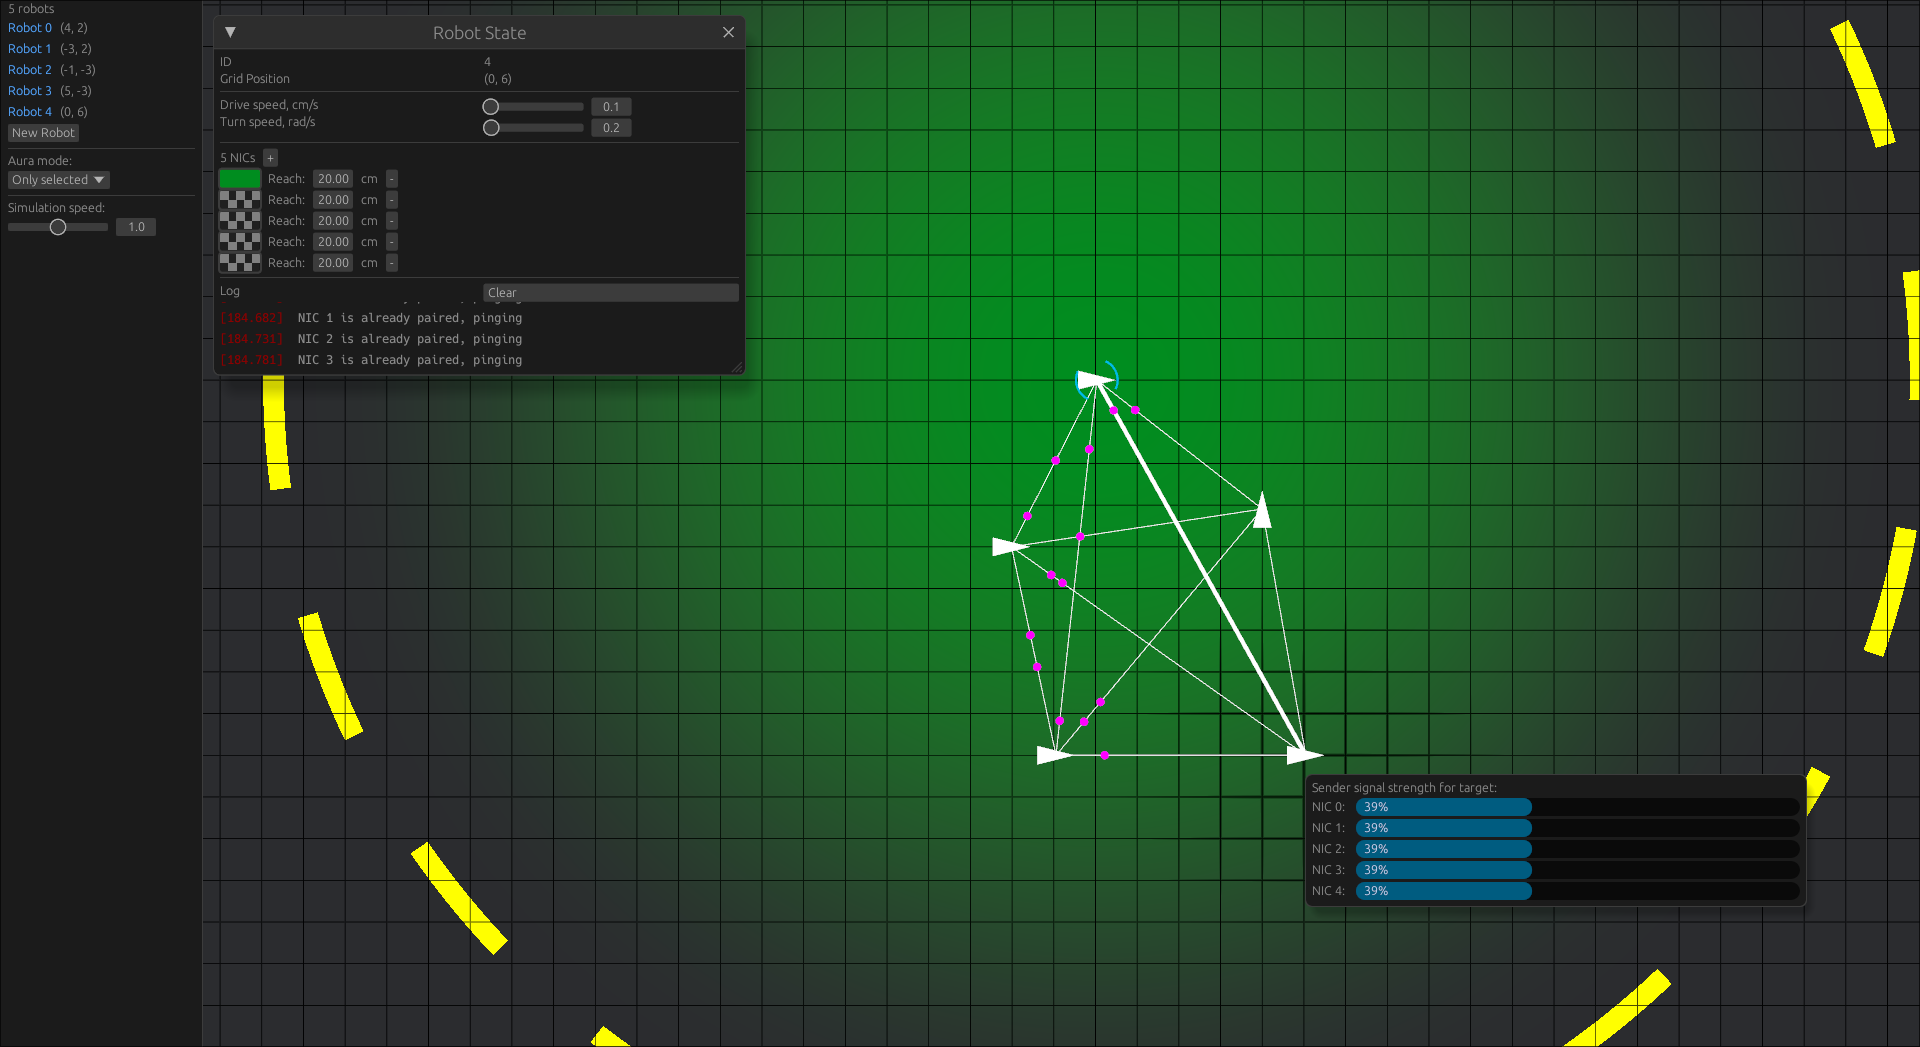
\includegraphics[width=\linewidth]{simulator-connections}
	\caption{Меш-сеть, представленная на рис. \ref{fig:connections}, реализованная внутри симулятора. Каждый робот имеет четыре виртуальных интерфейса, которые позволяют им установить соединение с каждым из соседей. Также на рисунке видна аура и пунктирная окружность вокруг верхнего робота, показывающая радиус действия его радио-интерфейсов; индикатор уровня сигнала, показывающий, что связь между верхним и нижним-правым роботом имеет уровень 39\%. Также видны кружочки на соединениях: это радио-сообщения, летящие между роботами, которые были отправлены, но еще не доставлены.}
  \label{fig:simulator-connections}
\end{figure}

\section{Ограничение памяти в микроконтроллерах}

Многие embedded-системы имеют очень маленькие лимиты оперативной
памяти и других ресурсов, особенно по сравнению с обычными компьютерами.
Например, на Raspberry Pi Pico,
который является приоритетной платформой для этого проекта
(или в микроконтроллере RP2040, на котором он основан),
есть 264KB оперативной памяти
и только 2MB flash-памяти~\cite{raspberrypi2021}.
(из которых можно использовать 1MB, если есть цель использовать OTA-обновление).

Из-за этого, при разработке интерфейсов есть приоритет --
использовать как можно меньше оперативной памяти.
Это можно увидеть в некоторых архитектурных решениях:
например, при сканировании Wi-Fi сетей,
возвращается не \texttt{Vec} найденных сетей -- 
потому что тогда нужно было бы использовать динамическую память,
и можно было бы вызвать атаку \emph{Denial-of-Service},
создав очень много сетей.
Вместо этого, метод сканирования принимает указатель на буфер,
в который он сохраняет информацию о сетях:
если доступных сетей больше, чем размер буфера,
то только первые несколько сетей сохраняются в буфер,
а остальные игнорируются.

Аналогично, многие решения по архитектуре приложения
принимаются во время компиляции, а не во время выполнения.
Так, в прошивке есть фиксированное число Wi-Fi модулей,
которые может поддерживать один робот,
и после компиляции нельзя подключить к RPi Pico больше модулей.
(Меньше -- можно, потому что все операции с Wi-Fi модулем могут возвращать ошибку,
и одна из возможных ошибок -- что модуль завис или не подключен. Но проверка модулей
занимает время, которое возможно было бы лучше сэкономить.)

В случае, если этого будет не достаточно для реализации физического кода,
можно выполнить \emph{hardware offloading}:
по умолчанию модули ESP-01 используются как <<черный ящик,>>
и общение с ними происходит только с помощью AT-команд.
Однако процессор ESP8266 содержит 50KB оперативной памяти,
а к тому же поддерживает до 16MB программной памяти через SPI.
Можно написать особенную прошивку для этих модулей,
которая выносит некоторые аспекты работы с сетью
за пределы кода основного контроллера,
и вместо этого основной контроллер будет посылать более высокоуровневые
команды для ESP,
тем самым экономя программную память для этих более сложных операций.

Это также полезно, потому что это повышает количество ядер процессора,
которые доступны для различных операций:
в RPi Pico доступно два ядра,
и если использовать ядра ESP8266,
то всего в системе будет 6 ядер.
Они ограниченны в своих способностях для коммуникации:
если один ESP хочет передать сообщение другому,
то в наивном режиме он должен дождаться,
пока RPi не спросит его о новых событиях,
и только после этого RPi передаст это сообщение другому ESP.
Можно использовать более сложную схему, 
где разные участники шины могут отправлять сообщения друг другу
без участия центрального контроллера
(так работает шина PCI Express),
но это более сложно:
так или иначе, весь этот подход требует написания особенной прошивки
для ESP-01,
что может быть затруднительно --
данный симулятор не поддерживает такого,
и сделать поддержку -- значит фактически реализовывать виртуальную машину
для каждого типа микроконтроллеров.

Наконец, если ресурсов микроконтроллеров совсем не хватает,
то можно просто  использовать более дорогой контроллер,
например Raspberry Pi Zero:
это уже полноценный Linux-компьютер с 512MB оперативной памяти;
по сравнению с микроконтроллерами это позволит запускать
очень сложные программы.

\section{Архитектура симулятора}

Поскольку Rust используется как основной язык разработки,
то для графического интерфейса и управления состоянием используется Bevy -- игровой движок на основе модели ECS
(\emph{Entity-Component-System}).
В этой модели существуют сущности (\emph{Entity}),
которые имеют лишь уникальный идентификатор.
К ним привязаны один или несколько компонентов
(\emph{Component}), которые описывают какое-то состояние:
например, в симуляторе используются компоненты,
которые обозначают, что данная сущность является роботом,
который в данный момент двигается от одной клетки к другой.
Наконец, при работе вызываются системы (\emph{System}) --
функции, которые обрабатывают и изменяют данные
в компонентах.

Эта архитектура похожа на ту, которая используется в более популярных
игровых движках вроде Unity~\cite{unity} и Godot;
однако там компоненты и системы
объединяются в одну сущность
(в Unity эта сущность называется \texttt{MonoBehaviour}).
Этот дизайн работает хуже в ситуациях,
когда один код должен действовать над несколькими разными объектами
(например, в симуляциях радио в этом проекте)
и часто требует создания дополнительных виртуальных объектов в игровом мире
для такой координации.

Общие типы сущностей, которые представлены в ECS -- 
роботы, их радио-модули,
соединения между роботами
и сообщения в полете.

\subsection{Сущность: Робот}

Для визуализации, робот имеет \emph{Mesh2d} и \emph{ColorMaterial}:
он отображается как белый треугольник.
Он также содержит \emph{RobotProps},
которые определяют базовые характеристики робота
(такие как скорость движения и поворота),
и \emph{RobotState}: 
его текущее состояние, в том числе
положение, направление движения
и каналы коммуникации с фоновыми потоками,
которые реализуют основную логику поведения.

При создании робота в симуляторе запускается два фоновых потока:
один -- для кода шасси
и один -- для кода радио-модуля.
Это сделано так, чтобы две задачи были незавиг от друга,
чтобы можно было менять поведение шасси без изменения радио-протокола.

Робот имеет два состояния: \emph{IdleRobot} и \emph{BusyRobot};
они представлены дополнительными компонентами.
Когда робот находится в состоянии \emph{IdleRobot},
он готов начать движение
(линейное или вращение).
Когда он начинает движение,
то к нему добавляется компонент,
который выполняет анимацию движения,
а сам робот становится \emph{BusyRobot}
(потому что он не может начать новое движение,
пока он не завершит предыдущее).
Наконец, когда робот завершает движение,
то компонент анимации удаляется,
а робот возвращает в состояние \emph{IdleRobot};
параллельно с этим
в фоновый поток отправляется сообщение,
которое разрешает скрипту шасси продолжить исполнение.

\subsection{Сущность: Интерфейс}

У каждого робота по умолчанию есть приемник,
который физически представлен как Wi-Fi AP.
Однако у него также может быть переменное число передатчиков:
каждый из них будет представлен отдельной сущностью,
которая следит за положением своего робота.

Такая сущность имеет настройки:
какой радиус действия у этой антенны есть,
какого цвета показывать ауру вокруг нее,
а также -- есть ли соединение с другим роботом,
и если да, то какой сущностью это соединение представлено.

\subsection{Сущность: Сообщение}

Для симуляции сложных консенсусных протоколов
может быть полезно иметь задержку между отправкой сообщения
и получением его,
а также разрешить пользователю вручную перехватывать и удалять сообщения в полете.
Для этого, вместо того чтобы сообщения доставлялись моментально после отправки,
они получают физическую форму в виде сущности-сообщения.
Сообщения показываются на экране как фиолетовые кружочки,
которые двигаются с постоянной скоростью к своему целевому роботу.
Когда сообщение оказывается близко к роботу,
то сама сущность сообщения удаляется,
а сообщение передается в очередь,
из которой скрипт данного робота может прочитать его.

\chapter{Разработка алгоритмов маршрутизации}

После создания симулятора,
поверх него можно реализовать алгоритмы маршрутизации.
Поскольку целью является использовать этот код на микроконтроллере,
нужно использовать алгоритмы, которые не будут требовать высокого
количества оперативной памяти.

По мере работы над этим проектом,
стала очевидна необходимость нескольких функций,
которые не входили в изначальное техзадание,
но которые очень полезны для удобной отладки скриптов роботов.
Поэтому, к симулятору добавили несколько функций,
которые облегчают эту отладку --
эти функции не доступны на аппаратной платформе.

\begin{itemize}
  \item Каждый робот имеет свой собственный лог,
  в который код может записывать, <<о чем он думает>>: 
  например, куда робот собирается поехать,
  какие соединения установлены у него,
  или какие сообщения он получил или отправил.
  На аппаратной платформе эта функция заменяется на заглушку, которая не делает ничего,
  и из-за этого компилятор может удалить весь код, который вызывает ее.
  \item Состояние симулятора (расположение роботов, количество и свойства их сетевых интерфейсов
  и существующие подключения) можно сохранить в файл.
  Это позволяет настроить какой-то конкретный сценарий,
  а затем тестировать его с различными изменениями кода.
  \item Чтобы более внимательно рассмотреть детали какой-то конкретной транзакции,
  можно поставить точку останова (\emph{breakpoint}) на определенные действия робота,
  такие как отправка или получение сообщения.
  Как только скрипт робота отправляет эту команду,
  симулятор ставится на паузу,
  и в этот момент можно внимательно рассмотреть логи,
  чтобы понять, что это поведение правильное.
  Также, для очень высокоскоростных симуляций,
  есть кнопка, которая позволяет выполнить определенное количество шагов симуляции:
  обычно симуляция работает со скоростью 60 кадров в секунду,
  поэтому посмотреть состояние на один-два кадра в будущее бывает сложно.
  \item В большой сети может быть сложно отследить, что происходит между большим количеством роботов,
  поэтому также добавлено окно, которое показывает все сообщения,
  которые были отправлены кем-либо в беспроводной сети.
  Такое окно показывает полную историю радио-коммуникации,
  с помощью которой можно отследить историю распространения одного конкретного факта по сети.  
\end{itemize}

Самый простой тип протокола -- \emph{flooding} (<<заливка>> или <<заполнение>>):
когда у одного из узлов сети появляется какая-то новая информация,
этот узел отправляет ее всем своим соседям, у которых этой информации пока что нет.
Затем, каждый из соседей повторяет это, пока информация у узла и у его непосредственных соседей
не будет одинаковой;
в этот момент данный узел завершает обработку этого пакета.
Слегка более сложная схема -- \emph{controlled flooding} -- игнорирует сообщение,
если оно уже было получено небольшое время назад (для этого
используется циклический буфер)~\cite{rahman2004controlled}.
Такие алгоритмы пригодны в ситуациях,
когда нужно распространить какую-то информацию по всей сети;
например, если нужно выполнить OTA-обновление прошивки микроконтроллеров.
Однако этот алгооритм имеет недостатки,
связанные с тем, что вся сеть будет получать одно и то же сообщение,
даже если этой части сети не интересно получать такое сообщение.

Flooding также иногда используется как компонент более сложных алгоритмов:
например, link-state (описанный ниже) подразумевает,
что каждый узел знает расстояние от себя до целевого узла,
и для этого при запуске сети каждый узел собирает информацию о своих ближайших соседях
и затем отправляет копию этой информации всем своим соседям;
каждый узел делает так и постепенно собирает более полную карту сети.
Этот алгоритм является версией flooding, которая часто известна как \emph{gossipping}
(<<сплетничать>>): узлы передают друг другу не точную копию какой-то информации,
а видоизмененную форму (карту своих соседей, дополненную слухами от соседей своих соседей),
что аналогично тому, как в группе общения распространяются сплетни.


Более сложные алгоритмы маршрутизации,
используемые и в проводных сетях,
чаще всего делятся на два типа:
\emph{link-state routing} и \emph{distance-vector routing}.

В link-state, каждый роутер имеет информацию про карту всей сети~\cite{arpanet_routing}.
Эта карта распространяется между роутерами с помощью flooding:
сначала каждый роутер говорит своим соседям обо всех своих ближайших соседях,
а затем каждый получатель добавляет к карте информацию о своих соседях,
и таким образом постепенно выстраивается полная карта всей сети.
После этого, если какой-то роутер хочет послать информацию какому-то другому роутеру,
то он строит маршрут с помощью своей собственной карты.
Что происходит дальше -- зависит от конкретного алгоритма:
в некоторых (например, \emph{Dynamic Source Routing}, DSR), этот желаемый маршрут вкладывается в заголовок пакета,
и остальные роутеры просто направляют пакет по этому маршруту,
и если какой-то шаг маршрута становится невозможным, то пакет просто удаляется
(этот подход работает хорошо в сетях, где маршруты редко становятся неверными,
как например в проводных сетях внутри здания).
В других алгоритмах, первый роутер просто отправляет свой пакет
по тому из своих соединений, которое указано первым в своем запланированном маршруте.
Следующий роутер будет использовать свою собственную карту, чтобы построить маршрут опять -- 
такой подход требует больше вычислений,
но работает лучше в ситуациях, когда маршруты могут прерываться неожиданно,
и эта информация не сразу распространяется по сети.

Чтобы каждый роутер не должен был хранить полную карту всей сети,
используется distance-vector: другой основной подход к маршрутизации.
Каждый роутер хранит меньшее количество информации:
ему нужно иметь только список (в жаргоне программирования, вектор) расстояний от себя до других роутеров в сети~\cite{rfc1058}.
Как и в link-state, каждый роутер обменивается этой информацией со своими соседями,
и соседи обновляют свое понимание сети в зависимости от этого;
алгоритм считается завершенным, когда каждый роутер получил стабильное понимание сети
и больше не обновляет свои векторы расстояний.

Алгоритмы типа distance-vector лучше подходят для беспроводных меш-сетей,
потому что роутеры не должны хранить полную карту всей сети (что занимает много памяти).
В частности, Zigbee -- протокол, который часто используется в IoT-устройствах ввиду своего низкого
энергопотребления --
основан на \emph{Ad-hoc On-Demand Distance Vector Routing} (AODV),
который был первый раз описан в 1999 году~\cite{perkins1999aodv}
и стандартизирован в RFC 3561~\cite{rfc3561}.
В AODV роутеры обмениваются информацией только в том случае,
если у них уже нет маршрута до какого-либо узла:
это минимизирует потребление памяти,
но увеличивает задержку для первого пакета для нового узла.

\section{Реализация в симуляторе}

Чтобы показать работоспособность симулятора,
на основе него необходимо реализовать хотя бы самый простой из этих алгоритмов -- flooding.
Он будет полезен в начальной фазе задачи мультиагентного планирования,
где все агенты получают одну и ту же информацию
по поводу той задачи, которую они решают.
Однако для простоты в этом конкретном проекте лучше обмениваться какой-то информацией,
которая присуща самим роботам.

В практической задаче это может быть какой-то факт об окружающей среде
(<<зарядная станция находится на координатах (13, 56)>>),
или какая-то команда, которая актуальна для всех узлов
(<<как можно быстрее, все роботы должны вернуться на станцию>>).
Однако такие факты находятся в области ответственности кода шасси,
который не хочется усложнять раньше времени.
Вместо этого, можно использовать другой подход,
с помощью которого можно будет наглядно увидеть, какая информация доступна конкретному роботу:
у них теперь есть цветовой индикатор,
и код шасси может менять его.

У каждого робота добавляется кнопка публикации этого цвета.
При нажатии на нее, робот сначала спрашивает своих подключенных соседей,
какой цвет сейчас у них.
Затем, он отправляет свой цвет всем тем соседям,
чей цвет отличается от его собственного.
Они затем меняют свой цвет на переданный им
и затем повторяют то же самое.
Этот процесс можно увидеть по шагам на рис. \ref{wave1}, \ref{wave2}, \ref{wave3}, \ref{wave4}.

Такой подход приводит к тому,
что все узлы сети быстро договариваются поставить себе один и тот же цвет,
и после этого волна сообщений останавливается:
последнее важно, чтобы можно было отправить новую волну с новым цветом.

На основании этого алгоритма можно распространять другую информацию, например обновления прошивки и планы, --
надо просто передавать больше, чем три байта за сообщение.

\begin{figure}[p]
  \centering
  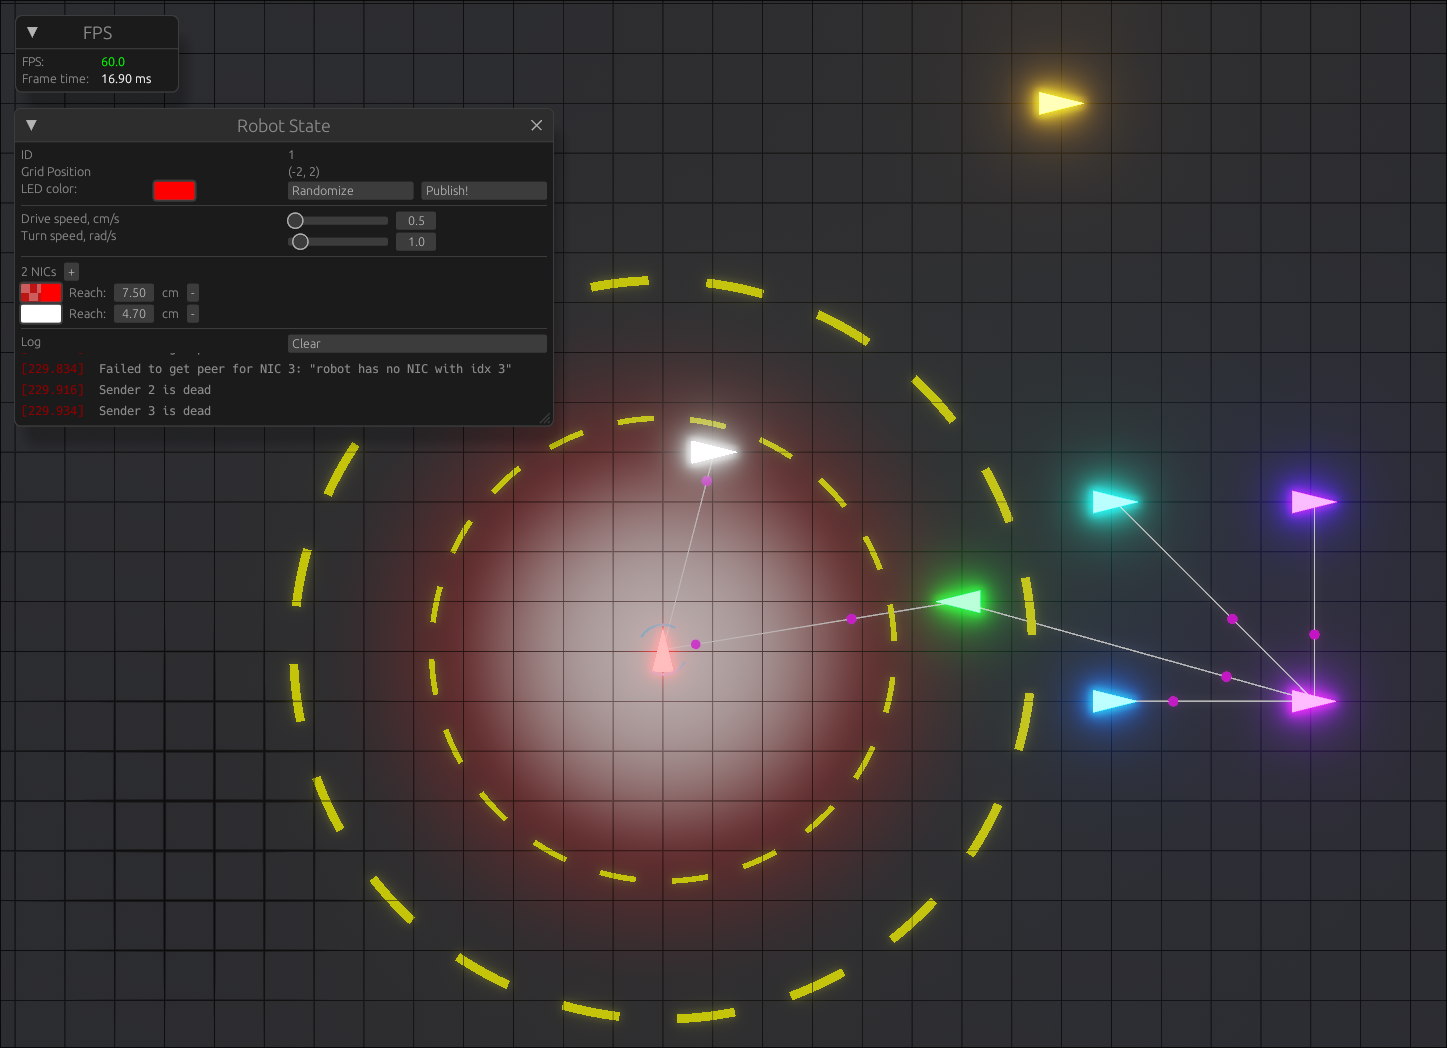
\includegraphics[width = 0.7\textwidth]{colors-1.png}
  \caption{Состояние симулятора до нажатия на кнопку публикации. Выделенный робот (слева)
  имеет красный цвет, а остальные роботы имеют случайно заданный цвет.}
  \label{wave1}
\end{figure}

\begin{figure}[p]
  \centering
  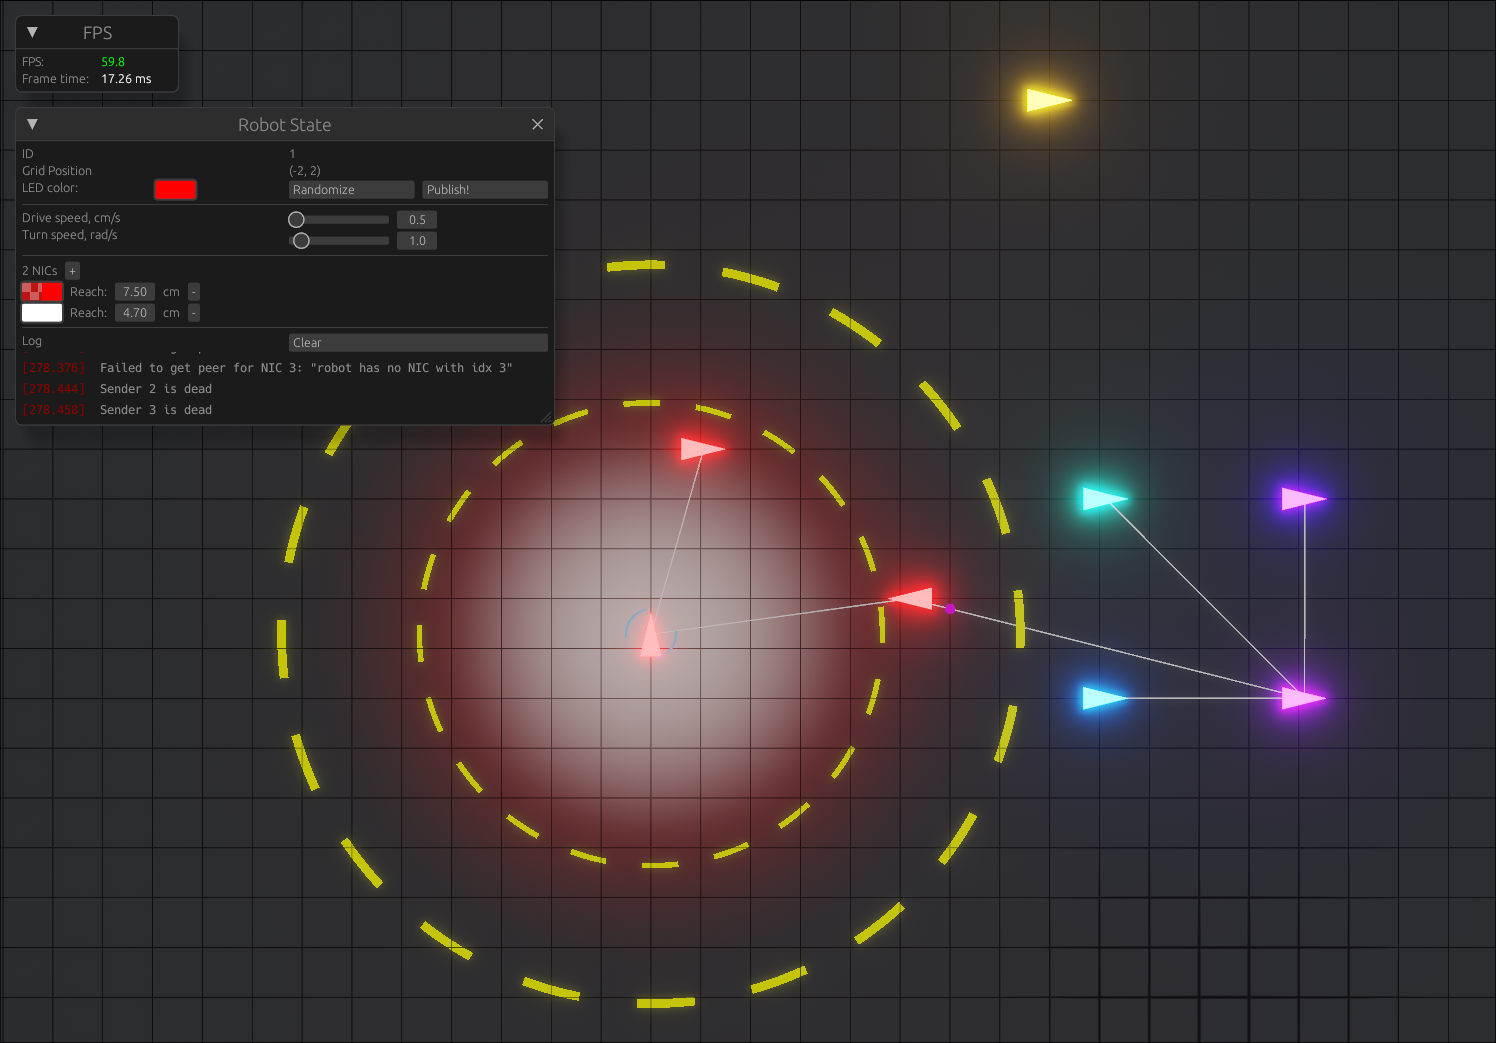
\includegraphics[width = 0.7\textwidth]{colors-2.png}
  \caption{Состояние симулятора после публикации цвета. Два робота, подключенных напрямую,
  получили новое сообщение и тоже стали красного цвета. После этого они начали рассылать свой цвет своим соседям.}
  \label{wave2}
\end{figure}

\begin{figure}[p]
  \centering
  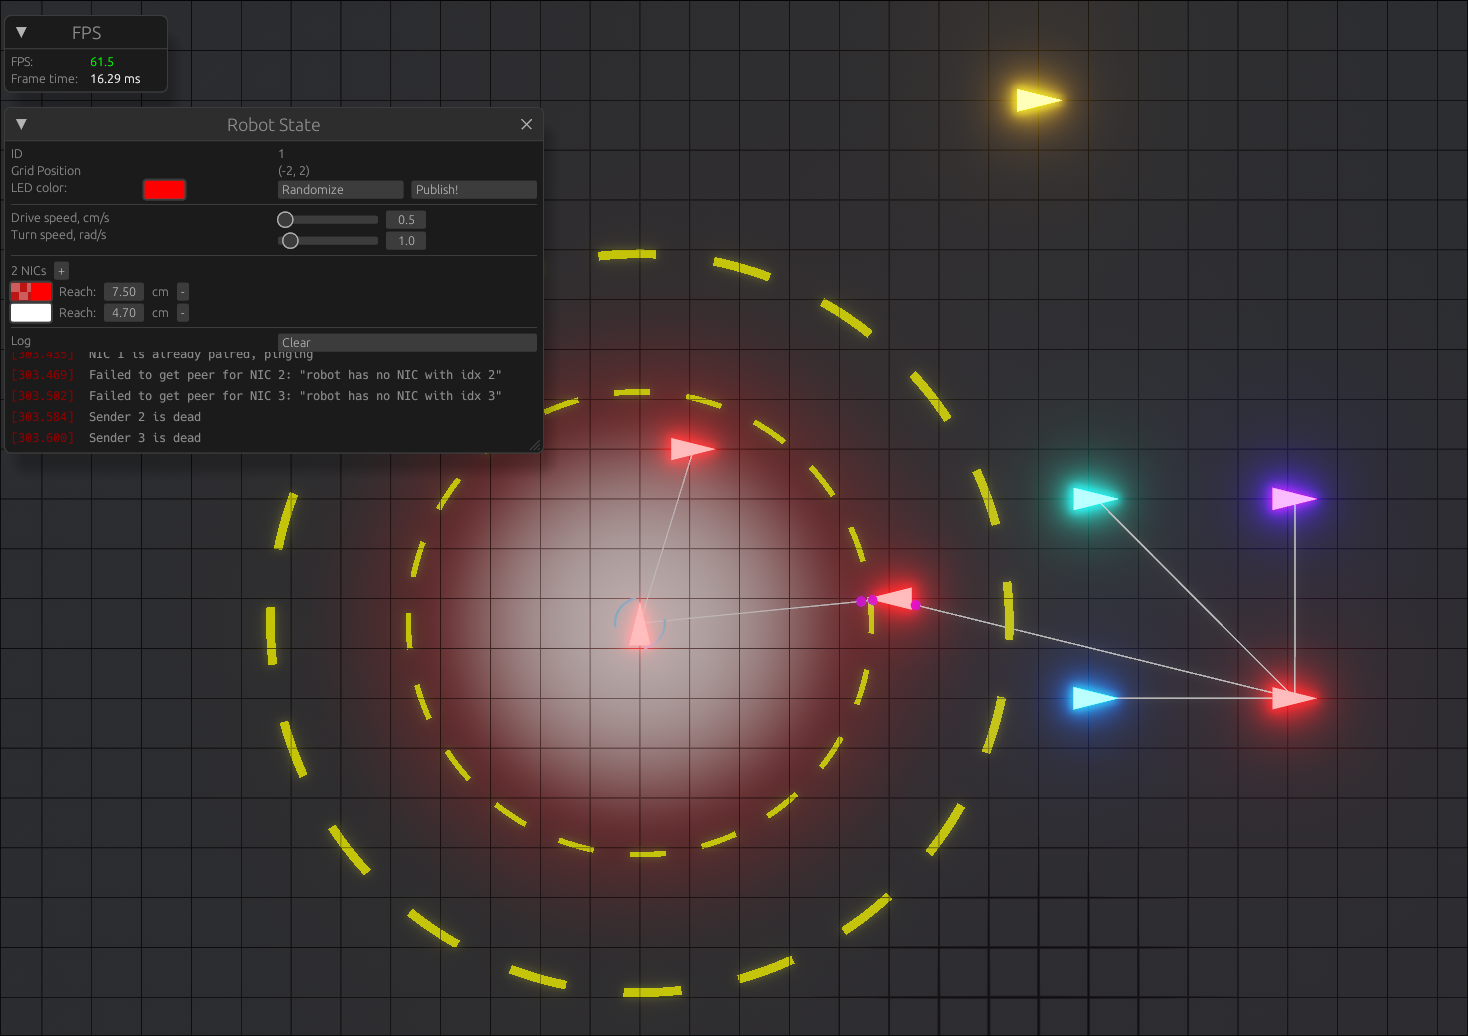
\includegraphics[width = 0.7\textwidth]{colors-3.png}
  \caption{Состояние симулятора после того, как информация о новом цвете прошла два шага. Она теперь достигла робота справа,
  который является центром для кластера трех роботов, которые подключены только к нему.}
  \label{wave3}
\end{figure}

\begin{figure}[p]
  \centering
  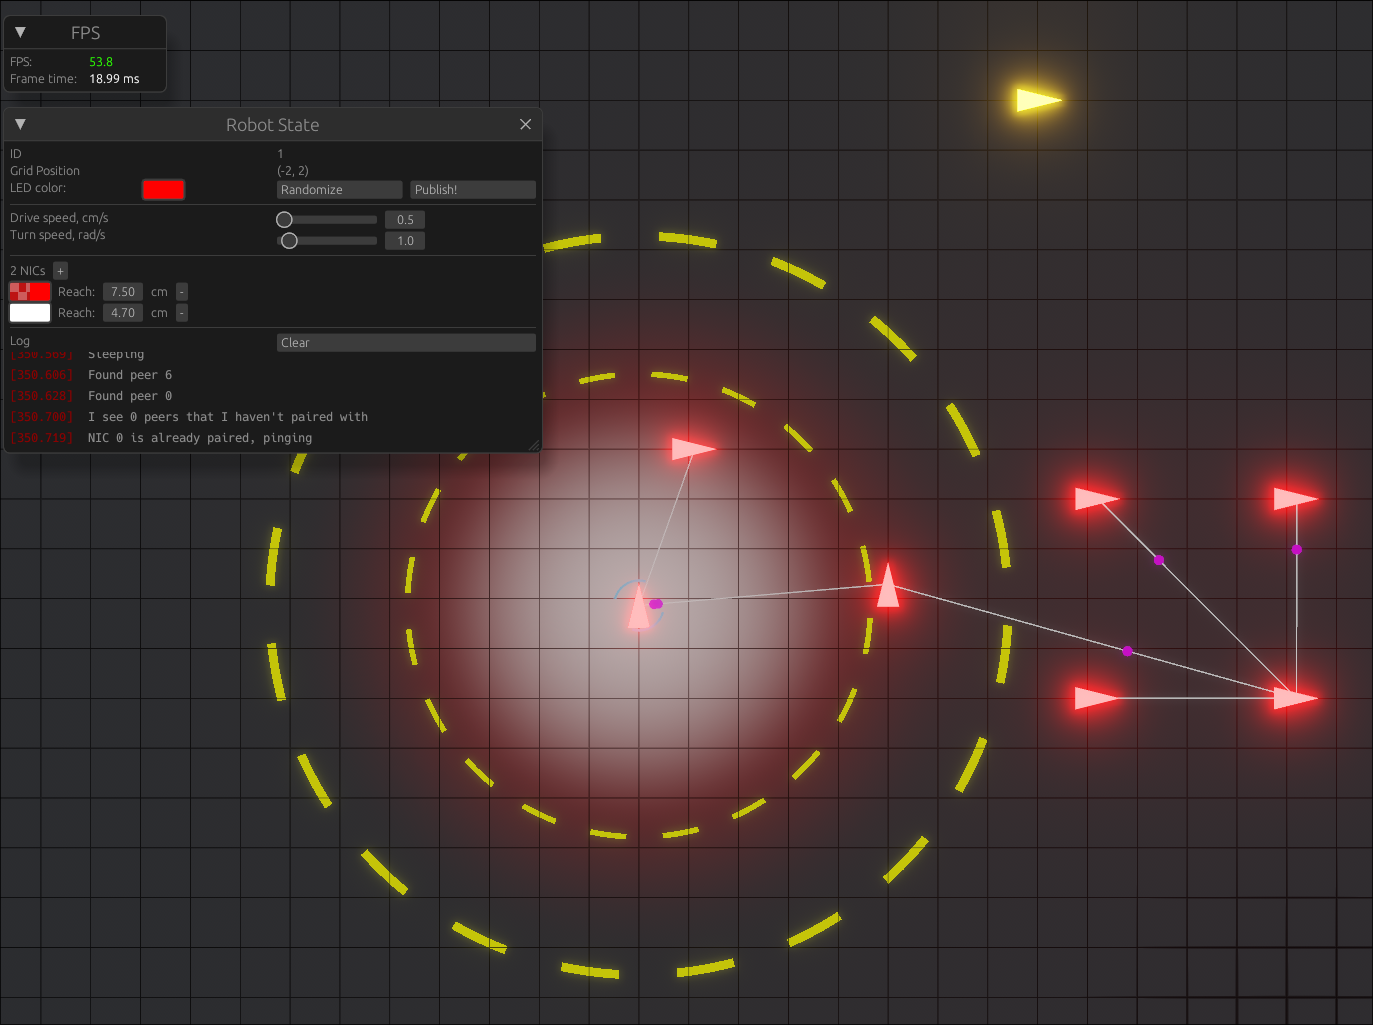
\includegraphics[width = 0.7\textwidth]{colors-4.png}
  \caption{Состояние симулятора после того, как все доступные роботы получили красный цвет. На этом действие алгоритма flood-алгоритма
  считается завершенным. Заметьте, что один робот,
  находящийся справа-сверху, не подключен ни к одному из этих, поэтому он не поменял свой цвет.}
  \label{wave4}
\end{figure}


\chapter*{Заключение}
\addcontentsline{toc}{chapter}{Заключение}

В данной работе был разработан симулятор для беспроводных мобильных меш-сетей
и продемонстрировали его API.
На основании этого API можно реализовать алгоритмы, которые будут
работать без изменения кода на виртуальной и аппаратной платформах.
Алгоритмы установления и поддержания связи внутри меш-сетей,
а также передачи данных по сети,
можно тестировать на симуляционной платформе,
а затем внедрять на физическую платформу без изменений.

По результатам обзора литературы обнаружены
некоторые ограничения текущей области исследований меш-сетей.
Одно из самых значительных --
в том, что более продвинутые симуляторы имеют интерфейс для кода,
несовместимый с интерфейсом для физических платформ.
Симулятор был разработан специально с акцентом на то,
чтобы API был унифицированным между кодом для физической платформы и для симулятора.
Это может позволить такому симулятору
стать основой для новых исследований
и прототипов меш-сетей.



\section*{Дальнейшая работа}

Этот симулятор предназначен в основном для интерактивного использования,
и он требует графического интерфейса.
Из-за этого он непригоден для ситуаций, когда GUI недоступен,
например на серверах или суперкомпьютерах.
Он также ограничен скоростью симуляции:
многие события требуют, чтобы хотя бы один кадр симуляции прошел
между действием и реакцией
(например: каждая транзакция между кодом радио-модуля
и виртуальным радио-модулем
требует одного кадра,
чтобы быть принятой симулятором.
Из-за этого,
даже если поставить скорость движения сообщений равной бесконечности,
то один робот все равно не сможет передать другому роботу
больше чем 60 сообщений в секунду.)

Эти ограничения связаны с конкретной реализацией симулятора
на основе игрового движка Bevy,
и в частности с тем, что для сообщений создаются отдельные сущности.
В будущем планируется создать опциональную реализацию,
которая будет работать без графического интерфейса
и обрабатывать события в дискретном времени:
с помощью этой версии можно будет симулировать гораздо более крупные сети.

Для использования в контексте задачи
мультиагентного планирования,
в симулятор будут добавлены
функции для создания дополнительных объектов,
с которыми могут взаимодействовать роботы:
это позволит отслеживать то,
как алгоритм маршрутизации и алгоритм планирования работают вместе.
В данный момент роботы могут только двигаться без ограничений,
и для более интересной задачи нужно будет добавить стены, которые препятствуют движению роботов,
радио-сигналов, или обоих.

Также следует добавить в симулятор
возможность менять код роботов во время исполнения, или
иметь больше одного скрипта:
в данный момент все роботы выполняют один и тот же скрипт.
Также следует добавить возможность добавлять свой собственный код:
сейчас код роботов компилируется вместе с кодом симулятора,
и его нельзя изменить без перекомпиляции всего проекта
(что сложно, если вы запускаете симулятор на веб-платформе).

Это можно сделать, например,
внедрив в симулятор виртуальную машину,
которая исполняет код для какой-то конкретной платформы,
и затем компилировать скрипт для робота для этой платформы.
Это может быть WebAssembly,
или (для симуляции ограниченных ресурсов)
это может быть виртуальная машина для какой-то RISC-архитектуры:
например, так работает компьютерная игра \emph{kartoffels}~\cite{kartoffels}.

Наконец, для того, чтобы можно было оценивать качество алгоритма
количественно, а не только качественно,
можно добавить в симулятор
сущности,
которые создают сообщения
и которые поглощают их
(так называемые \emph{source} или \emph{sink}).
Они могут измерять количество сообщений,
вошедших в сеть,
и количество успешно доставленных сообщений:
по сути это будет модуль для автоматического измерения процента доставленных пакетов
и метрик задержки передачи по сети.

Эти функции позволят данному симулятору достигнуть высокой степени 
расширяемости и универсальности,
и поэтому его можно будет использовать как основу для разработки
и прототипирования меш-сетей для мобильных роботов.

%Заключение является неотъемлемой частью любой работы. 

%Оно должно содержать краткие выводы по результатам исследования,
%отражающие новизну и практическую значимость работы, предложения по
%использованию ее результатов, оценку её эффективности и качества.

% \chapter{Ethical disclaimers}

% A disclaimer is a note of disclaimer of responsibility~\cite{kulyabov_2024_editorial_author-ethics_en}.
% For example, authors' statements about conflicts of interest, author contributions, acknowledgements, etc.

% Authors should not prepare these disclaimers as a numbered or unnumbered
% \mintinline{latex}{\chapter}%
% ; please use the special environments instead.

% \section{Author contributions}

% The Committee on Publication Ethics (COPE) draws attention to the problem of authorship \cite{cope_book_authorship_en}.
% The CRediT system (\url{https://credit.niso.org/}) is proposed to formalize author roles.
% The CRediT (Contributor Roles Taxonomy) offers 14 possible author roles \cite{holcombe_2019_contributorship-not-authorship_en}.
% This is not really a taxonomy, but a faceted classification. Author roles are not always independent in themselves.

% The following statements should be used \emph{Conceptualization, X.X. and Y.Y.; methodology, X.X.; software, X.X.; validation, X.X., Y.Y. and Z.Z.; formal analysis, X.X.; investigation, X.X.; resources, X.X.; data curation, X.X.; writing---original draft preparation, X.X.; writing---review and editing, X.X.; visualization, X.X.; supervision, X.X.; project administration, X.X.; funding acquisition, Y.Y.}
% Please add at the end of the statement:
% \emph{All authors have read and agreed to the published version of the manuscript.}

% This section has a special environment:
% \begin{minted}{latex}
% \begin{authorcontributions}
% …
% \end{authorcontributions}
% \end{minted}

% \section{Funding}

% Disclaimer \emph{funding} refers primarily to external funding if the research was externally initiated.
% If the research is entirely the initiative of the author's team, it is better to indicate gratitude for partial funding of some of the stages of the research in the \emph{Acknowledgments} section.
% The fact that the author's team has received external funding should be recorded in the disclaimer as a matter of course.
% When mentioning the sponsor, its exact data (name of the organization, grant number, etc.) and the country of its location should be specified (for example \emph{This research was funded by NAME OF FUNDER grant number XXX}).
% If there is any support, it is recommended to clarify in the \emph{Conflicts of interest} section at which stages of the research and how the support was used.
% If there is no external funding, it is written: \emph{This research received no external funding}.
% If it is impossible to obtain information from the authors about the source of funding, then write: \emph{Not specified}.

% This section has a special environment:
% \begin{minted}{latex}
% \begin{funding}
% …
% \end{funding}
% \end{minted}

% \section{Data availability statement}

% Data are particularly important in reproducible researches.
% The data availability statement tells the reader where the research data related to the article are located and under what conditions the data can be accessed.
% References to the dataset are also provided.

% If no new data is created or analyzed, please write:
% \emph{No new data were created or analyzed in this study. Data sharing is not applicable.}

% This section has a special environment:
% \begin{minted}{latex}
% \begin{dataavailability}
% …
% \end{dataavailability}
% \end{minted}

% \section{Conflicts of interest}

% This disclaimer must be included.

% Conflicts of interest can comment on various aspects, but usually the author's past or current employment is indicated.
% Grants (especially from for-profit companies) received not only by the author but also by the organization for which he or she works are indicated.
% If the author is associated with a sponsor, it is indicated where the research was conducted.

% If there is no conflict of interest, then the corresponding statement should also be included: \emph{The authors declare no conflict of interest}.

% This section has a special environment:
% \begin{minted}{latex}
% \begin{conflictsofinterest}
% …
% \end{conflictsofinterest}
% \end{minted}

% \section{Acknowledgments}

% Identification of funding sources and other support, and thanks to individuals and groups that assisted in the research and the preparation of the work should be included in an acknowledgment section, which is placed just before the reference section in your document.

% This section has a special environment:
% \begin{minted}{latex}
% \begin{acknowledgments}
% These are different acknowledgments.
% \end{acknowledgments}
% \end{minted}
% so that the information contained therein can be more easily collected during the article metadata extraction phase, and to ensure consistency in the spelling of the section heading.

% \chapter{Appendices}

% If your work needs an appendix, add it before the
% \mintinline{latex}{\end{document}}
% command at the conclusion of your source document.

% Start the appendix with the
% \mintinline{latex}{\appendix}
% command:
% \begin{minted}{latex}
% \appendix
% \end{minted}
% and note that in the appendix, sections are lettered, not numbered.

\vspace{\baselineskip}

% \begin{authorcontributions}
% %  Концептуализация, написание --- рецензирование и редактирование: Анна Владиславовна Королькова; методология, написание --- подготовка первоначального варианта: Дмитрий Сергеевич Кулябов.
% Концептуализация, написание --- подготовка первоначального варианта: Генералов Даниил Михайлович;
% руководство, написание --- рецензирование и редактирование: Андрей Николаевич Виноградов.
%   Все авторы прочитали и согласились с опубликованной версией рукописи.
% \end{authorcontributions}

% \begin{funding}
%   Данное исследование не получало внешнего финансирования.
% \end{funding}

% \begin{dataavailability}
%   В ходе исследования не было создано и проанализировано никаких новых данных. Совместное использование данных неприменимо.
% \end{dataavailability}

% \begin{conflictsofinterest}
%   Авторы заявляют об отсутствии конфликта интересов.
% \end{conflictsofinterest}

%\begin{acknowledgments}
%  Мы благодарим организаторов конференции за предоставленную возможность создать этот шаблон.
%\end{acknowledgments}

%%
%% Define the bibliography file to be used

% \printbibliography

\chapter*{Список литературы}
\addcontentsline{toc}{chapter}{Список литературы}


\printbibliography[heading=none]

%%
%% If your work has an appendix, this is the place to put it.
%\appendix

%\chapter{Онлайн-ресурсы}

%\begin{itemize}
%\item Overleaf: \url{https://www.overleaf.com/read/vjvjpsqrqjhj#86e97e}.
%\item Overleaf (russian): \url{https://www.overleaf.com/read/yjmkpnvgqzdk#bf8ccf}.
%\end{itemize}

\end{document}

%%% Local Variables:
%%% mode: LaTeX
%%% TeX-master: t
%%% End:
